\chapter{Ground-based lidar processing and simulator framework for comparing models and observations (ALCF~1.0)}

\vspace{-0.1cm}
\sffamily
\raggedright
\linespread{1.6}
Peter Kuma$^1$, Adrian J. McDonald$^1$, Olaf Morgenstern$^2$, Richard Querel$^3$, Israel Silber$^4$, and Connor J. Flynn$^5$
\footnotesize

\linespread{1}
\vspace{0.2cm}
\noindent
$^1$University of Canterbury, Christchurch, New Zealand\\
$^2$National Institute of Water \& Atmospheric Research (NIWA), Wellington, New Zealand\\
$^3$National Institute of Water \& Atmospheric Research (NIWA), Lauder, New Zealand\\
$^4$Department of Meteorology and Atmospheric Science, Pennsylvania State University, PA, USA\\
$^5$School of Meteorology, University of Oklahoma, Norman, OK, USA
\normalsize
\normalfont
\justify

\section*{Abstract}

Automatic lidars and ceilometers provide valuable information on cloud and aerosols, but have not been used systematically in the evaluation of GCMs and NWP models. Obstacles associated with the diversity of instruments, a lack of standardisation of data products and open processing tools mean that the value of the large ALC networks worldwide is not being realised. We discuss a tool, called the
Automatic Lidar and Ceilometer Framework (ALCF), that overcomes these problems and also includes a ground-based lidar simulator, which calculates the radiative transfer of laser radiation, and allows one-to-one comparison with models. Our ground-based lidar simulator is based on the Cloud Feedback Model Intercomparison
Project (CFMIP) Observation Simulator Package (COSP) which has been used extensively for spaceborne lidar intercomparisons. The ALCF
implements all steps needed to transform  and calibrate raw ALC data and create  simulated 
backscatter profiles for one-to-one comparison and complete statistical analysis of cloud. The framework supports multiple common
commercial ALCs (Vaisala CL31, CL51, Lufft CHM 15k and Sigma Space MiniMPL), reanalyses (JRA-55,
ERA5 and MERRA-2) and models (AMPS and the Unified Model). To demonstrate its
capabilities, we present case studies evaluating cloud in the
supported reanalyses and models using CL31, CL51, CHM 15k and MiniMPL
observations at three sites in New Zealand. We show that the reanalyses
and models generally underestimate cloud fraction and overestimate cloud albedo,
the common "too few too bright" problem.
If sufficiently high temporal resolution model output is available (better than 6 hourly), a direct comparison of
individual clouds is also possible. We demonstrate that the ALCF can be used as a generic
evaluation tool to examine cloud occurrence and cloud properties in reanalyses, NWP models and GCMs, potentially utilising the large amounts of ALC data already available. This tool  is likely to be  particularly useful for the analysis and improvement of low-level cloud simulations which are not well monitored from space. This has previously been identified as a critical deficiency in contemporary models, limiting the accuracy of weather forecasts and future climate projections.

\section{Introduction}

Automatic lidars and ceilometers (ALC) are active ground-based instruments
which emit laser pulses in the ultraviolet, visible or infrared (IR) part of the
electromagnetic spectrum and measure radiation backscattered from atmospheric
constituents such as cloud and fog liquid droplets and ice crystals, haze,
aerosol (particulate matter, ash) and atmospheric gases \citep{emeis2010}.
Vertical profiles of attenuated backscattered radiation can be produced
by measuring received power as a function of time elapsed between emitting the
pulse and receiving the backscattered radiation. Quantities such as
cloud base height (CBH) and a cloud mask
\citep{pal1992,wang2001,martucci2010,costa-suros2013,tricht2014,liu2015b,liu2015a,lewis2016,cromwell2019,silber2018}, aerosol optical depth
\citep{marenco1997,welton2000,welton2002,wiegner2012,wiegner2014,jin2015,dionisi2018} and boundary layer height
\citep{eresmaa2006,munkel2007,emeis2009,tsaknakis2011,milroy2012,knepp2017}
can be derived from the
backscatter profile. Lidars equipped with polarisation or multiple wavelengths
can also provide depolarisation ratio or colour ratio, respectively, which can be used
to infer cloud phase or particle types. Doppler lidars can measure wind
speed in the direction of the lidar orientation. ALCs are commonly deployed
at airports, where they provide CBH, fog and aerosol observations
needed for air traffic control. Large networks of up to
thousands of ACLs have been deployed worldwide: Cloudnet \citep{illingworth2007},
E-PROFILE \citep{illingworth2018}, EARLINET \citep{pappalardo2014},
ICENET \citep{cazorla2017}, MPLNET \citep{welton2006} and ARM \citep{stokes1994,campbell2002}.
The purpose of these networks is to observe cloud, fog, aerosol, air quality,
visibility and volcanic ash, provide input to numerical weather prediction (NWP)
model evaluation and
assimilation \citep{illingworth2015a,illingworth2018} and for climate studies.
These networks are usually composed of multiple types of ACLs, with Vaisala CL31,
CL51, Lufft (formerly Jenoptik) CHM 15k and Sigma Space MiniMPL
the most common.
Complex lidar data processing has been set up on some of these networks. Notably,
at the SIRTA site in France, lidar ratio (LR)
comparable with a lidar simulator \citep{chiriaco2018} is calculated 
as part of their "ReOBS" processing method. Intercomparison and calibration campaigns such as
CeiLinEx2015 \citep{mattis2016} and INTERACT-I(-II)
\citep{rosoldi2018,madonna2018} have been performed.
Lidar data processing involves a number of tasks such as resampling,
calibration, noise removal and cloud detection. Some of these are implemented
in the instrument firmware of ALCs. This, however, means that
lidar backscatter and detected cloud and cloud base are not comparable
between different instruments. In most cases the algorithms are not publicly
documented, making it impossible to compare the data with values from a model or a lidar simulator
without a systematic bias.

Atmospheric model evaluation is an ongoing task, and a critical
part of the model improvement process \citep{eyring2019,hourdin2017,schmidt2017}.
Traditionally, various types of observational and model datasets have been
utilised -- weather and climate station data, upper air soundings,
ground-based and satellite remote sensing datasets, and high-resolution model
simulations, amongst others.
Clouds are one of the most problematic phenomena in atmospheric models due
to their transient nature, high spatial and temporal variability, and
sensitivity to a complex combination of conditions such as relative humidity,
aerosols (presence of cloud condensation nuclei and ice nuclei), thermodynamic and dynamic conditions. At the same time, clouds have a very substantial
effect on the atmospheric shortwave and longwave radiation balance, and any
cloud misrepresentation has a strong effect on other components of the
model, limiting the ability to accurately represent past and present climate and
predict future climate \citep{zadra2018}.
An improved understanding of clouds and cloud feedbacks is one of the focuses of the Coupled Model
Intercomparison Project Phase 6 (CMIP6) \citep{eyring2016}, and comparison of model
cloud with observations is one of the key points of
the Cloud Feedback Model Intercomparison Project (CFMIP) \citep{webb2017}.
Satellite observations make up the majority of the data used to
evaluate model clouds. These include passive visible and IR
low earth orbit and geostationary radiometers measuring, among others,
features such as cloud cover, cloud top height (CTH), cloud top
temperature; passive microwave instruments measuring total column water; active
radars and lidars measuring cloud vertical profiles.
Ground-based remote
sensing instruments include radars, lidars, ceilometers, radiometers and sky
cameras. As pointed out by \cite{williams2017}, using a wide range of different
observational datasets including satellite and ground-based
for general circulation model (GCM) evaluation is important due to limitations of each dataset.

Model cloud is commonly represented by the mixing ratio of liquid and ice
and cloud fraction (CF) on every model grid cell and vertical level.
In addition some models provide the cloud droplet effective radius used in
radiative transfer calculations.
Remote sensing observations do not match the representation of the atmospheric
model fields directly because of their different resolutions, limited
field of view (FOV) and attenuation by atmospheric constituents before
reaching the instrument's receiver. Instrument simulators bridge this
gap by converting the model fields to quantities which emulate those measured by the instrument,
which can then be compared directly with observations. One such collection of instrument
simulators is the CFMIP
Observation Simulator Package (COSP) \citep{bodas-salcedo2011,swales2018},
which has been used for more than a decade for evaluation
of models using satellite, and more recently ground-based, observations.
The simulators in COSP include active instruments such as spaceborne and
ground-based radars: Cloud Profiling Radar (CPR) on CloudSat \citep{stephens2002}, Ka-band ARM Zenith Radar (KAZR); lidars:
Cloud-Aerosol Lidar Orthogonal Polarization (CALIOP) on CALIPSO \citep{winker2009}, Cloud-Aerosol Transport System (CATS) on ISS \citep{mcgill2015}, the Atmospheric Lidar (ATLID) on EarthCARE \citep{illingworth2015}; and spaceborne passive instruments:
ISCCP \citep{rossow1991}, MODIS \citep{parkinson2003} and MISR \citep{diner1998}. The more recent addition of ground-based radar
\citep{zhang2018} and lidar \citep{chiriaco2018,bastin2018}
opens up new possibilities to use the large amount of remote sensing data
obtained from ground-based active remote sensing instruments. In practice,
ground-based observational remote sensing data are not straightforward to use
without a substantial amount of additional processing. Some previous studies
have also compared models and ground-based radar and lidar observations
without the use of an instrument simulator \citep{bouniol2010,hansen2018}, though for the reasons identified above this is not advisable.

In this study we introduce a software package called the Automatic Lidar and Ceilometer
Framework (ALCF) for evaluating model cloud using ALC observations. It extends
and integrates the COSP lidar simulator \citep{chiriaco2006,chepfer2007,chepfer2008} with
pre- and post-processing steps, and allows the simulator to be run offline
on model output, instead of having to be integrated inside
the model. This makes it possible to compare ALC data at any location
without having to run the model with a specific configuration.
Multiple ALCs, reanalyses and model output formats are supported.
The original COSP lidar simulator was extended with Rayleigh and Mie scattering
at multiple lidar wavelengths. Observational ALC data from a number of common instruments can
be processed by re-sampling to a common resolution, removing noise, detecting cloud
and calculating statistics. The same steps can be performed on the simulated lidar data
from the model (the output of running COSP on the model data),
allowing for one-to-one comparison of model and observations.
A particular focus of our work was on applying the same processing steps on the
observed and simulated backscatter in order to
avoid biases. The ALCF is made available under an open source license (MIT)
at \url{https://alcf-lidar.github.io}, and as a permanent archive
of code and technical documentation on Zenodo at
\url{https://doi.org/10.5281/zenodo.3779518}.

A relatively small amount of other open source code is available for
ALC data processing. A lidar simulator has been developed as part of the Goddard
Satellite Data Simulator Unit (G-SDSU) \citep{G-SDSU}, a package based on the
instrument simulator package SDSU \citep{masunaga2010}. The Community
Intercomparison Suite (CIS) \citep{watson2016} allows for subsetting,
aggregation, co-location and plotting of mostly satellite
data with a focus on model--observations intercomparison. The STRAT lidar
data processing tools
are a collection of tools for conversion of raw ALC data, visualisation and feature
classification \citep{morille2007}.

Here, we provide an overview (Sect. \ref{sec:3:alcf}) and describe
the supported ALCs, reanalyses and models (Sect. \ref{sec:3:supported-alcs-reanalyses-and-models}).
We present a set of case studies at three sites in New Zealand (NZ)
(Sect. \ref{sec:3:case-studies}) to demonstrate the value of this new tool.
Furthermore, we describe the lidar simulator (Sect. \ref{sec:3:lidar-simulator}), observed and simulated lidar data processing steps (Sect. \ref{sec:3:lidar-data-processing}) and the results of the case studies
(Sect. \ref{sec:3:results}).

\section{Overview of operation of the Automatic Lidar and Ceilometer Framework (ALCF 1.0)}
\label{sec:3:alcf}

\begin{figure}[t]
\centering
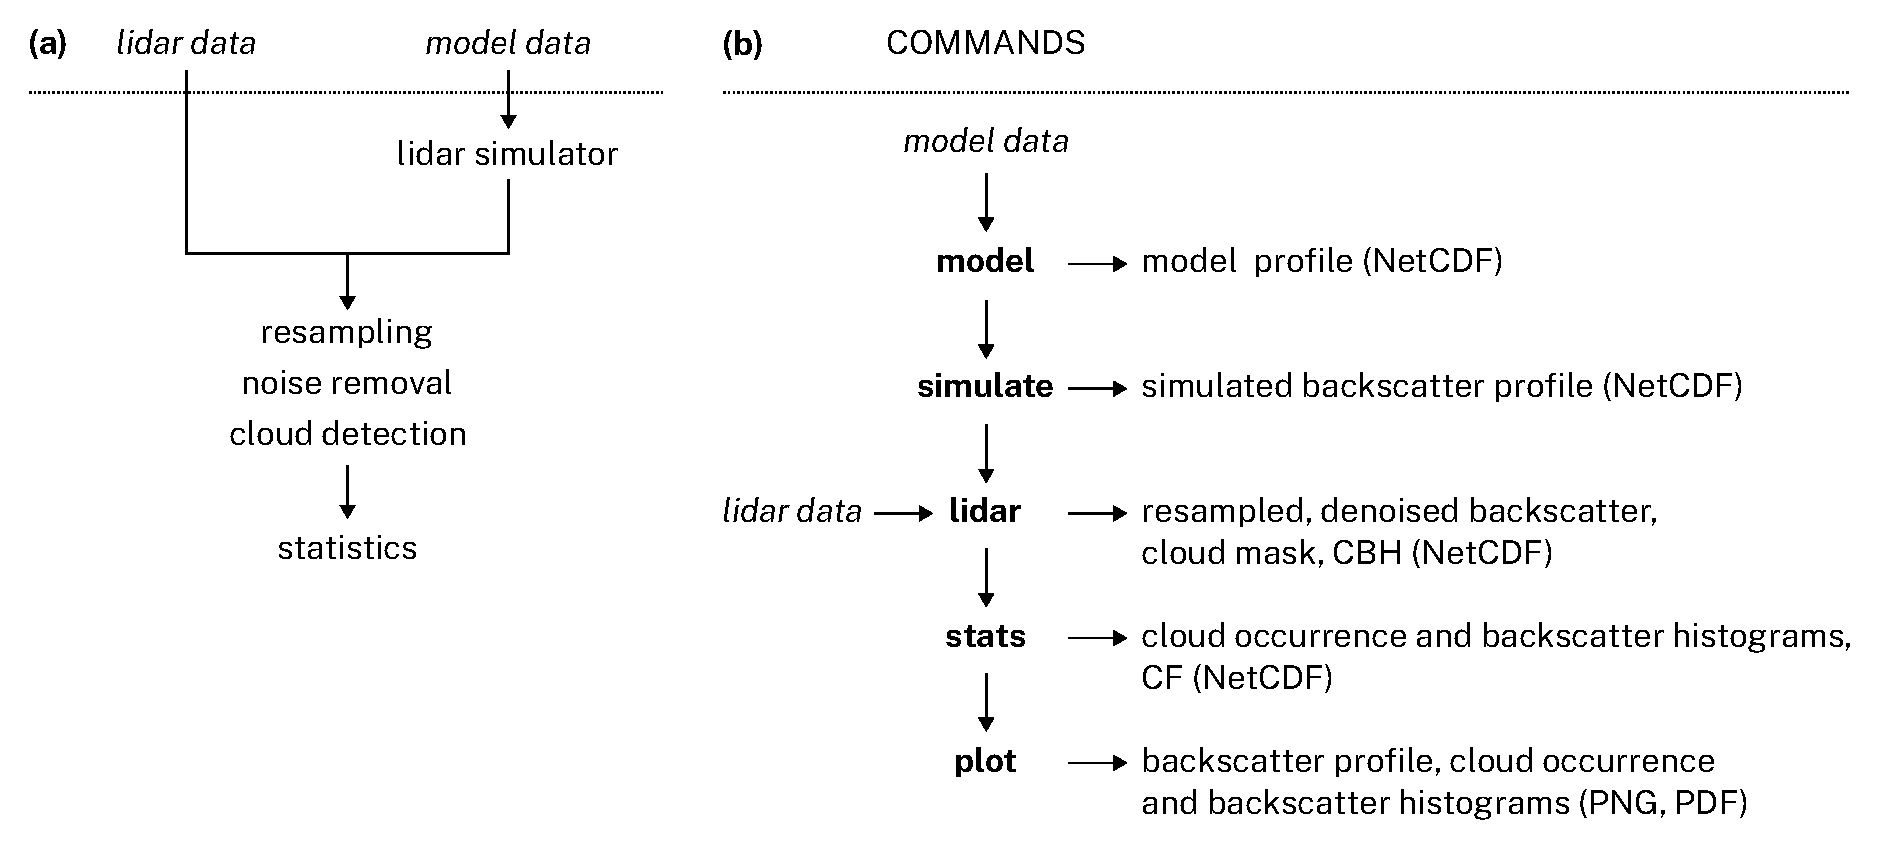
\includegraphics[width=\textwidth]{chapter3/fig/scheme.pdf}
\caption[Scheme showing the operation of the ALCF and the processing commands]{\textbf{(a)} Scheme showing the operation of the ALCF and \textbf{(b)} the processing commands.}
\label{fig:3:scheme}
\end{figure}

The ALCF performs the necessary
steps to simulate ALC backscatter based on 4-dimensional atmospheric fields
from reanalyses, NWP models and GCMs, and to transform the observed raw ALC
backscatter profiles to profiles comparable with the simulated profiles.
It does so by extracting 2-dimensional (time$\times$height) profiles from the
model data, performing radiative transfer calculations based on a modified COSP
lidar simulator (Sect. \ref{sec:3:lidar-simulator}),
absolute calibration and resampling of observed backscatter
to common resolution and performing comparable cloud detection on the simulated
and observed backscatter.
The framework
supports multiple common ALCs (Sect. \ref{sec:3:alcs}), reanalyses and models
(Sect. \ref{sec:3:reanalyses-and-models}).
The schematic in Fig. \ref{fig:3:scheme} illustrates this process
as well as the ALCF commands which perform the individual steps.
The following commands are implemented: \textbf{model}, \textbf{simulate},
\textbf{lidar}, \textbf{stats} and \textbf{plot}. The commands are normally
executed in a sequence, which is also implemented by a meta-command \textbf{auto},
which is equivalent to executing a sequence of commands. The commands are
described in detail in the technical documentation available online at
\url{https://alcf-lidar.github.io}, on Zenodo at \url{https://doi.org/10.5281/zenodo.3779518}
and in the Supplementary information. The physical basis is described here.

The \textbf{model}
command extracts 2-dimensional profiles of cloud liquid and ice content
(and other thermodynamic fields) from the supported NWP model, GCM and
reanalysis data (\textit{model data} in Fig. \ref{fig:3:scheme}) at a geographical point, along a ship track or a flight path.
The resulting profiles are recorded as NetCDF files. Sect. \ref{sec:3:reanalyses-and-models}
describes the supported reanalyses and models. The \textit{model data} can
be either in one of the supported model output formats,
or a new module for reading arbitrary model output can be written,
providing that the required atmospheric fields are present in the model output.
The required model fields are: per-level specific cloud liquid water content,
specific cloud ice water content, cloud fraction, geopotential height, temperature,
surface-level pressure and orography. No physical calculations are performed
by this command. The atmospheric profiles are extracted by a nearest-neighbour
selection.

The \textbf{simulate} command runs the lidar simulator described in Sect. \ref{sec:3:lidar-simulator}
on the extracted model data (the output of the \textbf{model} command) and produces simulated backscatter profiles. This command runs the COSP-derived lidar simulator, which performs
radiative transfer calculations of the laser radiation through the atmosphere.
The resulting simulated backscatter profiles are the output of this command.

The \textbf{lidar} command applies various processing algorithms on either
the simulated backscatter data (the output of the \textbf{simulate} command)
or the observed ALC data (\textit{lidar data} in Fig. \ref{fig:3:scheme})
(Sect. \ref{sec:3:lidar-data-processing}). The data are resampled
to increase the signal-to-noise ratio (SNR), noise is subtracted, LR is calculated,
a cloud mask is calculated by applying a cloud detection algorithm and CBH is determined
from the cloud mask. Absolute calibration (Sect. \ref{sec:3:backscatter-calibration})
can also be applied in this step by
multiplying the observed backscatter by a calibration coefficient. This is
important in order to obtain unbiased backscatter profiles comparable with the simulated
backscatter profiles. Sect. \ref{sec:3:alcs} describes the supported instruments.
The \textit{lidar data} can be in one of the supported instrument formats. If
the native instrument format is not NetCDF, it has to be converted from the native
format with the auxiliary command \textbf{convert} or one of the conversion
programs: cl2nc (Vaisala CL31, CL51), mpl2nc or SigmaMPL (Sigma Space MiniMPL).

The \textbf{stats} step calculates summary statistics from the output of the 
\textbf{lidar} command. These include CF, cloud occurrence by height,
backscatter histograms and the averages of LR and backscatter.

The \textbf{plot} command plots the backscatter profiles produced by the \textbf{lidar}
command (Fig. \ref{fig:3:examples}, \ref{fig:3:examples2}, \ref{fig:3:examples3}), and
the statistics produced by the \textbf{stats} command: cloud occurrence
(Fig. \ref{fig:3:case-studies}), backscatter histograms (Fig. \ref{fig:3:micro-backscatter})
and backscatter noise standard deviation histograms (Fig. \ref{fig:3:backscatter-sd-hist}).

\begin{table}[t]
\caption[Table of ALCs and their technical parameters]{Table of ALCs and their technical parameters. Power is calculated as Pulse$\times$Pulse Repetition Frequency (PRF).}
\label{tab:3:alcs}
\centering
\scalebox{0.68}{
\begin{tabular}{lllllllllll}
\hline
Instrument & $\lambda$ (nm) & Laser & Rate\footnotemark[1] (s) & Res.\footnotemark[2] (m) & Depol.\footnotemark[3] & Pulse\footnotemark[4] ($\mu$J) & Range\footnotemark[5] (km) & PRF (kHz) & Overlap\footnotemark[6] (m) & Power (mW)\\
\hline
CHM 15k & 1064 & Nd:YAG & 2--600 & 5 & no & 7--9 & 15.4 & 5--7 & 1000\footnotemark[7] & 48\\
CL31 & 910 & InGaAs & 2--120 & 10 & no & 1.2 & 7.7 & 10 & 70\footnotemark[7] & 12\\
CL51 & 910 & InGaAs & 6--120 & 10 & no & 3 & 15.4 & 6.5 & 230\footnotemark[8] & 20\\
MiniMPL & 532 & Nd:YAG & 1--900 & 5--75 & yes & 3--4 & 30.0 & 2.5 & 2000\footnotemark[8] & 9\\
\hline
\end{tabular}
}
\footnotesize
$^1$Sampling rate.
$^2$Vertical (range) resolution.
$^3$Depolarisation.
$^4$Pulse energy.
$^5$Maximum range.
$^6$Range of full overlap.
$^7$\cite{hopkin2019}.
$^8$\cite{madonna2018}.
\normalsize
\end{table}

\section{Supported input data: instruments, reanalyses and models}
\label{sec:3:supported-alcs-reanalyses-and-models}

\subsection{Instruments}
\label{sec:3:alcs}

The primary focus of the framework is to support common commercial ALCs.
Ceilometers are considered the most basic type of lidar \citep{emeis2010,kotthaus2016}
intended as commercial products designed for unattended operation.
They are used routinely to measure CBH, but most instruments also provide the
full vertical profiles of backscatter. Therefore, they are suitable for model
evaluation by comparing not only CBH, but also cloud occurrence as a function
of height. Their compact size and low cost make it possible to deploy a large
number of these instruments in different locations, or use them in unusual settings
such as mounted on ships \citep{klekociuk2019,kuma2020a}. Common off-the-shelf
ceilometers are
the Lufft CHM 15k, Vaisala CL31 and CL51.
Some lidars offer higher power
and therefore higher SNR, and capabilities not present in ceilometers such as
dual polarisation, multiple wavelengths, Doppler shift measurement and Raman scattering.
Below we describe ALCs supported by the framework and used in our case studies:
Lufft CHM 15k, Vaisala CL31 and CL51 and Sigma Space MiniMPL.
Table \ref{tab:3:alcs} lists selected parameters of the supported ALCs.

\textit{Lufft CHM 15k} (previously Jenoptik CHM 15k) is a ceilometer operating
at a wavelength of 1064 nm in the
near IR spectrum. The maximum range of the instrument is 15.4 km, vertical sampling
resolution 5 m and sampling rate up to 2 s. The wavelength in the near IR
spectrum ensures low molecular backscatter.
The instrument produces NetCDF files containing uncalibrated attenuated
backscatter profiles and various derived variables.

\textit{Vaisala CL31 and CL51} are ceilometers operating at a wavelength of 910
nm in the near IR spectrum. The maximum range of CL31 and CL51 is 7.7 km and 15.4 km
and the sampling rate is 2 and 6 s, respectively. The vertical resolution
is 10 m. The wavelength is characterised by relatively low molecular backscatter
(but higher than 1064 nm) and is affected by water vapour absorption
\citep{wiegner2015,wiegner2019}, which can cause additional absorption of about 
20\% in the mid-latitudes and 50\% in the tropics (see also Sect. \ref{sec:3:water-vapour-absorption}).
The instruments produce
data files containing uncalibrated attenuated backscatter which can be converted
to NetCDF (see cl2nc in the Code and data availability section).
The firmware configuration option "noise\_h2 off" results in backscatter
range correction to be selectively applied under a certain critical range
and above this range only if cloud is present \citep[Sect. 3.2]{kotthaus2016}.
This was the case with our case study dataset (Sect. \ref{sec:3:case-studies}).
We apply range correction on the uncorrected range gates during lidar
data processing. The critical range in CL51 is not documented, but was
determined as 6000 m based on an observed discontinuity.

\textit{Sigma Space (part of Hexagon) Mini Micro Pulse Lidar (MiniMPL)} \citep{spinhirne1993,campbell2002,flynn2007} is a
dual-polarisation micro pulse lidar (meaning that it uses a high pulse repetition rate (PRF) and low pulse power)
operating at a wavelength of 532 nm (green) in the visible spectrum. The maximum range of the
instrument is 30 km. The vertical resolution is up to 5 m and sampling rate up
to 1 s. The shorter wavelength is affected
by stronger molecular backscatter than 910 nm and 1064 nm.
The instrument can be housed in a protective enclosure, which makes it suitable
for deployment in a relatively harsh environment. A scanning head can be
mounted on the enclosure which provides configurable scanning by elevation
angle and azimuth. The instrument produces data files containing raw
backscatter which can be converted to NetCDF containing normalised relative
backscatter (NRB) with a vendor-provided tool SigmaMPL
(see also mpl2nc in the Code and data availability section).

\begin{table}
\caption[Reanalyses and models used in the case studies and some of their main
properties]{
Reanalyses and models used in the case studies and some of their main
properties. The temporal and horizontal grid resolution and vertical levels listed is the
resolution of the model output available. The horizontal grid resolution is determined at 45\unit{^\circ}S.
The internal resolution of the model may be different
(see Sect. \ref{sec:3:reanalyses-and-models} for details). The reanalyses and the
UM use regular longitude-latitude grids, while the AMPS horizontal grid is
regular in the South Pole stereographic projection.
}
\label{tab:3:models}
\centering
\scalebox{0.96}{
\begin{tabular}{llllllll}
\hline
Model/Grid & Type & Time resolution & Horizontal grid resolution & Vertical levels\\
\hline
AMPS/D01 & NWP & 3 h & 0.27\unit{^\circ}$\times$ 0.19\unit{^\circ} (21$\times$21 km) & 60\\
ERA5 & Reanalysis & 1 h & 0.25\unit{^\circ}$\times$0.25\unit{^\circ} (20$\times$28 km) & 37\\
JRA-55 & Reanalysis & 6 h & 1.25\unit{^\circ}$\times$1.25\unit{^\circ} (98$\times$139 km) & 37 \\
MERRA-2 & Reanalysis & 3 h & 0.625\unit{^\circ}$\times$0.50\unit{^\circ} (49$\times$56 km) & 72\\
UM (GA7.1)/N96 & GCM & 20 min. & 1.875\unit{^\circ}$\times$1.25\unit{^\circ} (147$\times$139 km) & 85\\
\hline
\end{tabular}
}
\end{table}

\subsection{Reanalyses and models}
\label{sec:3:reanalyses-and-models}

Below we briefly describe reanalyses and models\footnote{We use the term "reanalysis" when referring to ERA5, JRA-55 and MERRA-2 even though the reanalyses are based on atmospheric models. We use the term "model" when referring to AMPS and the UM, which are atmospheric models.} used in the case studies
presented here (Sect. \ref{sec:3:case-studies}). We used publicly available output from three reanalyses and one NWP model. In addition, we performed nudged GCM simulations with
high-temporal resolution output with the Unified Model (UM).
Table \ref{tab:3:models} lists some of the main properties of the reanalyses and
models.

\textit{The Antarctic Mesoscale Prediction System (AMPS)} \citep{powers2003}
is a limited-area NWP model based on the polar fifth-generation Pennsylvania State
University-National Center for Atmospheric Research Mesoscale Model (Polar MM5),
now known as the Polar Weather Research and Forecasting (WRF) model \citep{hines2008}.
The model serves operational and scientific needs in Antarctica, but its largest grid also covers the South Island of NZ.
AMPS forecasts are publicly available on the Earth System Grid
\citep{williams2009b}.
The forecasts are produced on several domains. The largest domain D01 used in the presented analysis covers
NZ and has horizontal grid spacing of approximately 21 km over NZ. The model uses 60 vertical levels. The model output is available
in 3-hourly intervals and initialised at 00:00 and 12:00 UTC. The initial and
boundary conditions are based on the Global Forecasting System (GFS) global
NWP model. AMPS assimilates local Antarctic observations from human-operated stations, automatic
weather stations (AWS), upper-air stations and satellites.

\textit{ERA5} \citep{era5} is a reanalysis produced by the European Centre
For Medium-Range Weather Forecasts (ECMWF) currently available for the time
period 1979 to present, with a plan to extend the time period to 1950.
The reanalysis is based on the global NWP model Integrated Forecast System (IFS)
version CY41R2. It uses a 4D-Var assimilation of station, satellite,
radiosonde, radar, aircraft, ship-based and buoy data. The model has 137
vertical levels. Atmospheric fields are interpolated from horizontal resolution
equivalent of 31 km and 137 model levels on regular longitude-latitude grid
of 0.25\unit{^\circ} and 37 pressure levels, and made available to the end-users.
In this analysis we use the hourly data on pressure and single levels.

\textit{Japanese 55-year reanalysis (JRA-55)} \citep{ebita2011,kobayashi2015,harada2016}
is a global reanalysis produced by the
Japan Meteorological Agency (JMA) and the Central Research Institute of Electric
Power Industry (CRIEPI) based on the JMA Global Spectral Model (GSM).
The reanalysis is available from 1958 onward.
The reanalysis is based on the JMA operational assimilation system.
JRA-55 uses a 4D-Var assimilation of surface, upper-air, satellite, ship-based
and aircraft observations. The model uses 60 vertical levels and a horizontal
grid with resolution approximately 60 km. In this analysis we
use the 1.25\unit{^\circ} isobaric analysis and forecast fields interpolated to
37 pressure levels.

\textit{Modern-Era Retrospective analysis for Research and Applications
(MERRA-2)} \citep{gelaro2017}
is a reanalysis produced by the NASA Global Modeling and Assimilation Office (GMAO).
The reanalysis is based on the Goddard Earth Observing System (GEOS) atmospheric
model. The model has approximately 0.5\unit{^\circ}$\times$0.65\unit{^\circ} horizontal
resolution and 72 vertical levels. It performs 3D-Var assimilation of
station, upper-air, satellite, ship-based and aircraft data in 6-hourly
cycles. In this analysis, we use the MERRA-2 3-hourly instantaneous
model-level assimilated meteorological fields (M2I3NVASM) version 5.12.4 product.

\textit{The UK Met Office Unified Model (UM)} \citep{walters2019}
is an atmospheric model for weather forecasting and climate projection
developed by the UK Met Office and the Unified Model Partnership. The UM is the atmospheric
component, called Global Atmosphere (GA), of the HadGEM3–GC3.1 GCM and the UKESM1
earth system model (ESM). In this analysis we performed custom nudged
runs of the UM \citep{telford2008} in the GA7.1 configuration with 20 min.
time step and output temporal resolution
on a New Zealand eScience Infrastructure (NeSI)/National Institute of Water \& Atmospheric Research (NIWA) supercomputer \citep{williams2016}.
The model was nudged to the ERA-Interim \citep{dee2011} atmospheric fields of horizontal wind speed and potential temperature and the HadISST sea surface temperature (SST) and sea ice dataset
\citep{rayner2003}. The model uses 85 vertical levels and a horizontal grid
resolution of 1.875\unit{^\circ}$\times$1.25\unit{^\circ}.

\section{Lidar simulator}
\label{sec:3:lidar-simulator}

The COSP lidar simulator Active Remote Sensing Simulator (ACTSIM) was
introduced by \cite{chiriaco2006} for the purpose
of deriving simulated CALIOP measurements \citep{chepfer2007,chepfer2008}.
The simulation is implemented by applying the lidar equation on model levels.
Scattering by cloud particles
and air molecules is calculated using the Mie and Rayleigh theory,
respectively. CALIOP operates at a wavelength of 532 nm, and
calculations in the original COSP simulator use this wavelength.
We implemented a small set of changes to the lidar simulator to support a
number of ALCs with different operating wavelengths.

\begin{table}[t]
\caption{Table of physical quantities.}
\label{tab:3:physical-quantities}
\centering
\scalebox{0.74}{
\begin{tabular}{llll}
\hline
Symbol & Name & Units & Expression\\
\hline
$\alpha_s$ ($\alpha_e$) & Volume scattering (extinction) coefficient & m$^{-1}$ & \\
$\Omega$ & Solid angle & sr & \\
$P_\pi(\theta)$ & Scattering phase function at angle $\theta$ & 1 & $\int_{4\pi} P_\pi (\theta) \mathrm{d}\Omega = 4\pi$\\
$\beta$ & Volume backscattering coefficient & m$^{-1}$sr$^{-1}$ & $\beta = \alpha_s P_\pi(\pi)/(4\pi)$\\
$N$ & Particle number concentration & m$^{-3}$ & \\
$n(r)$ & Number distribution of particle size & m$^{-4}$ & $N = \int_0^\infty n(r) \mathrm{d}r$ \\
$Q_s$ ($Q_e$) & Scattering (extinction) efficiency of spherical particles & 1 & $\alpha_s = Q_s \pi r^2 N$, $\alpha_e = Q_e \pi r^2 N$ \\
$Q_b$ & Backscattering efficiency of spherical particles & sr$^{-1}$ & $\beta = Q_b \pi r^2 N$ \\
$S$ & Lidar ratio (extinction-to-backscatter ratio) & sr & $S = \alpha_e/\beta$\\
$k$ & Backscatter-to-extinction ratio & sr$^{-1}$ & $k = 1/S$\\
$r_\text{eff}$ & Effective radius & m & $r_\text{eff} = \int_0^\infty r^3 n(r)\mathrm{d}r/\int_0^\infty r^2 n(r)\mathrm{d}r$\\
$\sigma_\text{eff}$ & Effective standard deviation & m & $\sigma_\text{eff} = \left(\int_0^\infty (r - r_\text{eff})^2 r^2 n(r) \mathrm{d}r\right)/\left(\int_0^\infty r^2 n(r) \mathrm{d}r\right)$\\
$k_B$ & Boltzmann constant & \unit{JK^{-1}} & $k_B \approx 1.38\times 10^{-23}$ \unit{JK^{-1}}\\
$p$ & Atmospheric pressure & Pa & \\
$T$ & Atmospheric temperature & K & \\
$\rho$ & Liquid (or ice) density & \unit{kg.m^{-3}} & \\
$\rho_\text{air}$ & Air density & \unit{kg.m^{-3}} & \\
$q$ & Cloud liquid (or ice) mass mixing ratio & 1 & \\
\hline
\end{tabular}
}
\end{table}

The lidar equation \citep{emeis2010} is based on the radiative transfer equation \citep{goody1995,liou2002,petty2006,zdunkowski2007},
which relates transmission of radiation to scattering, emission and absorption
in media such as the atmosphere. The lidar equation assumes laser radiation
passes through a
horizontally homogeneous atmosphere where it is absorbed and scattered. A fraction
of laser radiation is scattered back to the instrument and reaches the receiver.
Scattering and absorption in the
atmosphere is determined by its constituents -- gases, liquid droplets,
ice crystals and aerosol particles.
Atmospheric model output typically contains 4-dimensional fields of mass mixing ratios
of liquid and ice and CF. The lidar equation can be applied on these
output fields to simulate the backscattered radiation received by the instrument.
Table \ref{tab:3:physical-quantities} lists physical quantities used in the
following sections. Here, we use radiative transfer notation similar to
\cite{petty2006} and the notation of the original lidar simulator
\citep{chiriaco2006}.

\subsection{Rayleigh and Mie scattering}
\label{sec:3:rayleigh-and-mie-scattering}

The Rayleigh volume backscattering coefficient $\beta_\text{mol}$ (\unit{m^{-1}sr^{-1}}) in ACTSIM is parametrised by the following equation
(Eq. (8) in \cite{chiriaco2006}):

\begin{align}
\beta_\text{mol} = \frac{p}{k_BT}(5.45\times 10^{-32})\left(\frac{\lambda}{550 \mathrm{nm}}\right)^{-4.09}
= \frac{p}{k_BT}C_\text{mol} ,
\end{align}

\noindent where for lidar wavelength $\lambda$ = 532 nm, $C_\text{mol} = 6.2446\times 10^{-32}$
; $k_B$ is the Boltzmann constant $k_B \approx 1.38\times 10^{-23}$ \unit{JK^{-1}},
$p$ is the atmospheric pressure and $T$ is the atmospheric temperature.
We multiply this equation by $\exp(4.09(\log(532) - \log(\lambda)))$ (where the value of $\lambda$ is in nm)
to get molecular backscatter for wavelengths other than 532 nm, which allows us to support multiple commercially available instruments.
The strength of molecular backscattering is usually lower than
backscattering from clouds for the relevant wavelengths.

The lidar signal at visible or near IR wavelengths is scattered by
atmospheric constituents of similar size in the Mie scattering regime \citep{mie1908}.
In the most simple approximation,
one can assume spherical dielectric particles. The scattering from these particles depends on the
relative size of the wavelength and the (spherical) particle radius $r$, expressed by the
dimensionless size parameter $x$:

\begin{align}
x = \frac{2\pi r}{\lambda} .
\end{align}

While the wavelength is approximately constant during the operation of the lidar\footnote{The actual lidar wavelength is not constant and is characterised
by a central wavelength and width. The central wavelength may fluctuate with
temperature \citep{wiegner2015}.},
the particle size comes from a distribution of sizes, typically approximated
in NWP models and GCMs by a Gamma or log-normal distribution with a given mean
and standard deviation. Some models provide the mean as effective radius $r_\text{eff}$.
If the effective radius is not provided by the model, the lidar simulator
assumes a value $r_\text{eff}$ = 30 $\mu$m by default, which is the value assumed by the original ACTSIM
simulator.

In order to support multiple laser wavelengths, it is necessary
to calculate backscattering efficiency due to scattering by a distribution
of particle sizes. We use the computer code MIEV developed by Warren J Wiscombe
\citep{wiscombe1979,wiscombe1980} to
calculate backscattering efficiency for a range of the size parameter
$x$ and integrate for a distribution of particle sizes. The resulting
pre-calculated LR (extinction-to-backscatter ratio) as a function
of the effective radius is included in the lidar simulator for fast lookup
during the simulation.

Cloud droplet and ice crystal size distribution parameters are an important assumption
in lidar simulation due to the dependence of Mie scattering on the ratio of
wavelength and particle size (the size parameter $x$). NWP models and GCMs
traditionally use the effective radius $r_\text{eff}$ and effective standard
deviation $\sigma_\text{eff}$ (or an equivalent parameter such as effective variance $\nu_\text{eff}$)
 to parametrise this distribution. Knowledge of the real distribution is likely highly
uncertain due to a large variety of clouds occurring globally and the limited
ability to predict microphysical cloud properties in models. In this section
we introduce theoretical assumptions used in the lidar simulator based on established
definitions of the effective radius and effective standard deviation and two
common distributions.
\cite{edwards1996} discuss the effective radius in the context of model radiation
schemes, and we will primarily follow the definitions detailed in \cite{chang2001} and
\cite{petty2011}. The practical result of this section (and the corresponding
offline code) is pre-calculated backscatter-to-extinction ratios as a function of
the effective radius in the form of a lookup table included in the lidar
simulator, and used in the online calculations. The offline code
is provided and can be re-used for calculation of the necessary lookup tables for
different lidar wavelengths, should the user of the code want to support another
instrument.

The effective radius $r_\text{eff}$ and effective standard deviation $\sigma_\text{eff}$
are defined by:

\begin{equation}
\label{eq:eff}
r_\text{eff} = \frac{\int_0^\infty r^3 n(r)\mathrm{d}r}{\int_0^\infty r^2 n(r)\mathrm{d}r}, \quad
\sigma_\text{eff}^2 = \frac{\int_0^\infty (r - r_\text{eff})^2 r^2 n(r) \mathrm{d}r}{\int_0^\infty r^2 n(r) \mathrm{d}r} ,
\end{equation}

where $n(r)$ is the probability density function (PDF) of the distribution.
Here, we follow \cite{petty2011}, who define the effective variance
$\nu_\text{eff}$ which relates to $\sigma_\text{eff}$
by $\nu_\text{eff} = \sigma_\text{eff}^2 / r_\text{eff}^2$.
Due to lack of knowledge about the real distribution of particle radii, it has to be modelled by a
theoretical distribution, such as a log-normal or Gamma distribution.
The original ACTSIM simulator assumes a log-normal distribution \citep{chiriaco2006}
with the PDF:

\begin{equation}
n(r) \propto \frac{1}{r}\exp\left(-\frac{(\log r - \mu)^2}{2\sigma^2}\right) ,
\end{equation}

where $\mu$ and $\sigma$ are the mean and the standard
deviation of the corresponding normal distribution, respectively.
\cite{chiriaco2006} use the value of $\sigma = \log(1.2) = 0.18$ "for ice clouds" (the value
for liquid cloud does not appear to be documented). In our parametrisation
we used a combination of $r_\text{eff}$ and $\sigma_\text{eff}$
to constrain the theoretical distribution, where the effective standard deviation $\sigma_\text{eff}$ was assumed to
be one fourth of the effective radius $r_\text{eff}$. This choice is approximately
consistent with $\sigma = \log(1.2) = 0.18$ at $r_\text{eff}$ = 20 $\mu$m
(see Table \ref{tab:3:size-dist}, described below). In future updates, the values
could be based on in situ studies of size distribution or taken from the
atmospheric model output if available.

\begin{table}
\caption[Table of sensitivity tests]{Table of sensitivity tests of theoretical distribution assumption,
effective radius $r_\text{eff}$ and effective standard deviation
$\sigma_\text{eff}$ of the cloud droplet/ice crystal size distribution.
$\mu$ and $\sigma$ are the mean and standard deviation
of a normal distribution corresponding to the log-normal distribution,
calculated numerically from $r_\text{eff}$ and $\sigma_\text{eff}$.
$\mu_*$ and $\sigma_*$ are the actual mean and standard deviation of the
distribution (calculated numerically).}
\label{tab:3:size-dist}
\centering
\begin{tabular}{lllllll}
\hline
Distribution & $r_\text{eff}$ ($\mu$m) & $\sigma_\text{eff}$ ($\mu$m) & $\mu$ & $\sigma$ & $\mu_*$ ($\mu$m) & $\sigma_*$ ($\mu$m) \\
\hline
log-normal & 20 & 10 & 2.44 & 0.47 & 12.76 & 6.26 \\
log-normal & 20 & 5 & 2.84 & 0.25 & 17.72 & 4.43 \\
log-normal & 10 & 5 & 1.74 & 0.47 & 6.40 & 3.20 \\
Gamma & 20 & 10 & & & 9.98 & 7.00 \\
Gamma & 20 & 5 & & & 17.50 & 4.68 \\
Gamma & 10 & 5 & & & 5.00 & 3.54 \\
\hline
\end{tabular}
\end{table}

From the expression for the n-th moment of the log-normal distribution
$E[X^n] = \exp(n\mu + n^2\frac{\sigma^2}{2})$ and Equation \eqref{eq:eff}
we calculate $r_\text{eff}$ and $\sigma_\text{eff}$ of the log-normal distribution:

\begin{align}
r_\text{eff} &= \frac{E[r^3]}{E[r^2]} = \exp(\mu + \frac{5}{2}\sigma^2) ,\\
\sigma_\text{eff}^2 &= \frac{E[(r-r_\text{eff})^2r^2]}{E[r^2]} = \frac{E[r^4] - 2E[r^3]r_\text{eff} + r_\text{eff}^2E[r^2]}{E[r^2]} = \frac{\exp(4\mu + 8\sigma^2) - \exp(4\mu + 7\sigma^2)}{\exp(2\mu + 2\sigma^2)} = \nonumber\\
&= \exp(2\mu + 6\sigma^2) - \exp(2\mu + 5\sigma^2).
\end{align}

We find $\mu$ and $\sigma$ for given $r_\text{eff}$ and $\sigma_\text{eff}$
numerically by root-finding using the equations above. In practice,
we find that the root-finding converges well for $r_\text{eff}$ between 5
and 50 $\mu$m, which is the range mostly likely to be applicable in practice.

The Gamma distribution follows the PDF:

\begin{equation}
n(r) \propto r^{(1 - 3\nu_\text{eff})/\nu_\text{eff}}\exp\left(-\frac{r}{r_\text{eff}\nu_\text{eff}}\right)
\end{equation}

(see e.g. Eq. 13 in \cite{petty2011}
or Eq. 1 in \cite{breon2005}). In this case, the distribution depends explicitly on $r_\text{eff}$ and
$\sigma_\text{eff}$, and as such does not require numerical root-finding.

\begin{figure}[t]
\centering
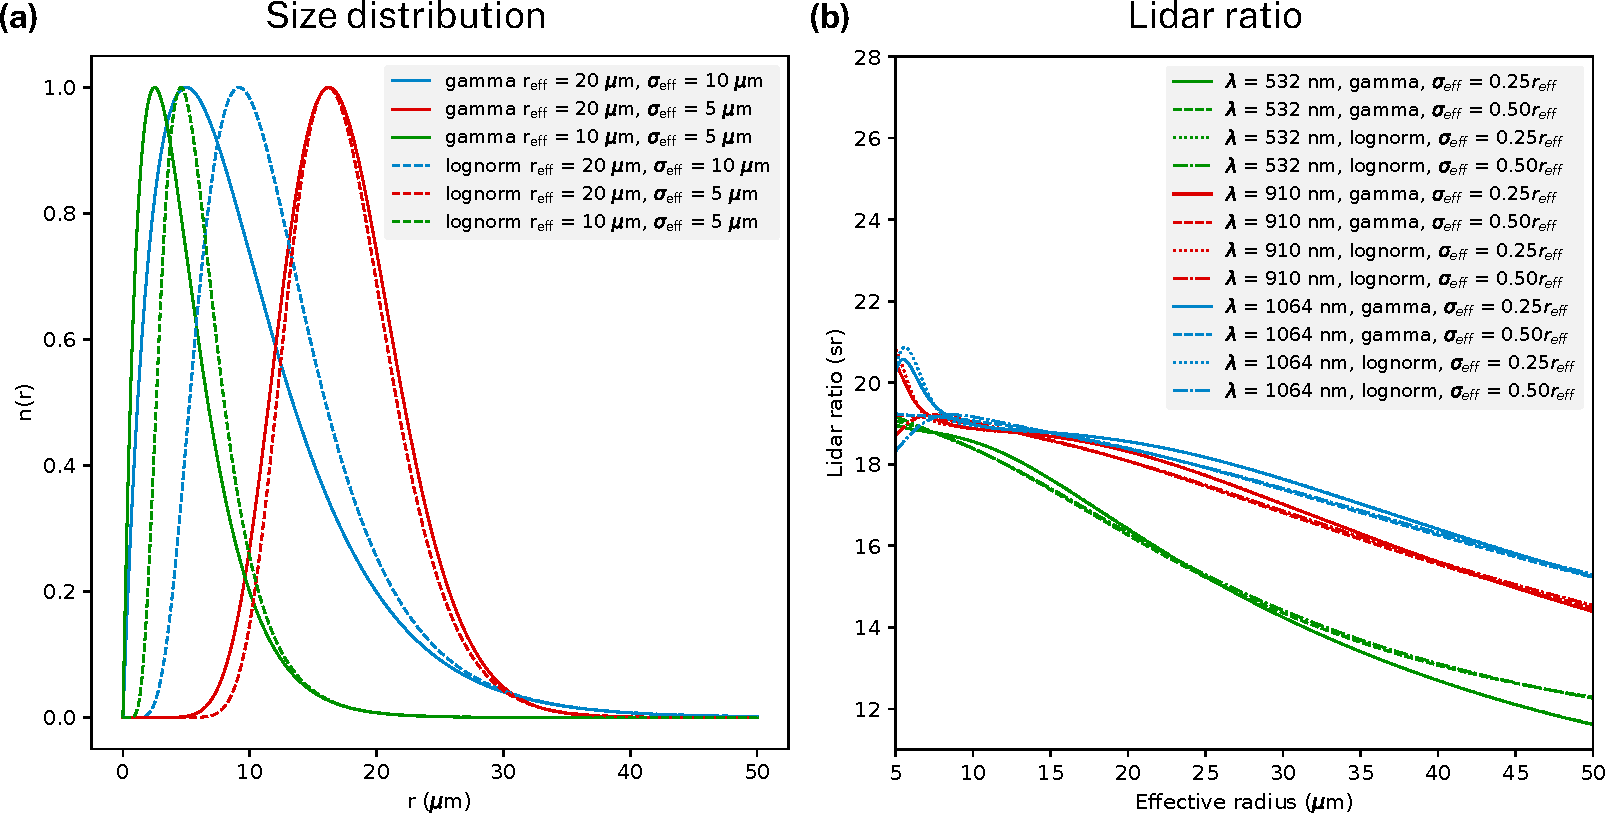
\includegraphics[width=\textwidth]{chapter3/fig/size_dist.pdf}
\caption[Theoretical distributions of cloud droplet radius]{
\textbf{(a)} Theoretical distributions of cloud droplet radius based on
the log-normal and Gamma distributions parametrised
by multiple choices of the effective radius $r_\text{eff}$ and effective standard deviation
$\sigma_\text{eff}$. \textbf{(b)} Lidar ratio (LR) as a function of effective
radius calculated for different theoretical cloud droplet size
distributions, laser wavelengths and effective standard deviation ratios.
}
\label{fig:3:size-dist}
\end{figure}

Figure \ref{fig:3:size-dist}a shows the log-normal and Gamma distributions
calculated for a number of $r_\text{eff}$ and $\sigma_\text{eff}$ values,
and Table \ref{tab:3:size-dist} summarises properties of these distributions.
The actual mean and standard deviation of the distributions do no necessarily
correspond well with the effective radius and effective standard deviation.

In ACTSIM, the volume extinction coefficient $\alpha_e$
is calculated by integrating the extinction by individual particles over the
particle size distribution:

\begin{equation}
\alpha_e = 
\int_0^\infty Q_e\pi r^2 n(r) \mathrm{d}r \approx
Q_e\pi\int_0^\infty r^2 n(r) \mathrm{d}r =
Q_e \frac{3q\rho_\text{air}}{4\rho r_\text{eff}} ,
\end{equation}

assuming approximately constant extinction efficiency $Q_e \approx 2$ (which is approximately true for the interesting range of $r_\text{eff}$ and laser wavelengths), and using the
relationship between the cloud liquid (or ice) mass mixing ratio $q$
and $\int_0^\infty r^2 n(r) \mathrm{d}r$:

\begin{equation}
q\rho_\text{air} = \int_0^\infty \frac{4}{3}\pi r^3 \rho n(r)\mathrm{d}r = 
\frac{4}{3}\pi\rho\int_0^\infty r^3 n(r) \mathrm{d}r =
\frac{4}{3}\pi\rho r_\text{eff}\int_0^\infty r^2 n(r) \mathrm{d}r ,
\end{equation}

where $\rho$ and $\rho_\text{air}$ are the densities of liquid water (or ice)
and air, respectively.

Likewise, the volume backscatter coefficient
from particles $\beta_p$ is calculated by integrating backscattering by
individual particles over the particle size distribution:

\begin{equation}
\beta_p =
\int_0^\infty Q_s \pi r^2 \frac{P_\pi(\pi)}{4\pi} n(r) \mathrm{d}r .
\end{equation}

where $Q_s$ is scattering efficiency and $P_\pi(\pi)$ is scattering phase function
at 180$^\circ$.
Since the normalisation of $n(r)$ is not known until the online phase of calculation,
the backscatter-to-extinction ratio from particles $k_p = \beta/\alpha_e$ can be
calculated offline instead (the requirement for normalisation of $n(r)$ is
avoided by appearing in both the numerator and denominator):

\begin{equation}
k_p = \beta_p/\alpha_e = \frac{\int_0^\infty Q_s r^2 P_\pi(\pi)/(4\pi) n(r) \mathrm{d}r}{\int_0^\infty Q_e r^2 n(r) \mathrm{d}r} .
\end{equation}

We pre-calculate this integral numerically for a permissible interval of
$r_\text{eff}$ (5--50 \unit{\mu m}) at 500 evenly spaced wavelengths,
and store the result as a lookup table for the online phase.
The integral in the numerator is numerically hard to calculate due
to strong dependency of $P_\pi(\pi)$ on $r$.
Figure \ref{fig:3:size-dist}b
shows LR as a function of $r_\text{eff}$, calculated
for log-normal and Gamma particle size distributions with $\sigma_\text{eff}
= 0.25 r_\text{eff}$ and $\sigma_\text{eff} = 0.5 r_\text{eff}$.
This corresponds to the lookup table we use in the online phase
of the lidar simulator. As can be seen in Fig. \ref{fig:3:size-dist},
LR depends only weakly on the choice of the distribution type and the effective standard
deviation ratio.

\subsection{Cloud overlap and cloud fraction}

Model cloud is defined by the liquid and ice mass mixing ratio and cloud
fraction in each atmospheric layer. The lidar simulator simulates radiation
passing vertically at a random location within the grid cell. Therefore,
it is necessary to generate a random vertical cloud overlap based on the cloud
fraction in each layer, as the overlap is not defined explicitly in the model output.
Two common methods of generating overlap are the
random and maximum--random overlap \citep{geleyn1979}. In the random overlap method,
each layer is either cloudy or clear with
a probability given by CF, independent of other layers.
The maximum--random overlap assumes that adjacent layers with non-zero CF are maximally
overlapped, whereas layers separated by zero CF layers are randomly overlapped.
COSP implements cloud overlap generation in the
Subgrid Cloud Overlap Profile Sampler (SCOPS)
\citep{klein1999,webb2001,chepfer2008}. The ALC lidar simulator uses SCOPS to
generate 10 random subcolumns for each profile, using the maximum--random
overlap assumption as the default setting of a user-configurable option.
The backscatter profile and cloud occurrence can be plotted for any subcolumn.
Due to the random nature of the overlap, the backscatter profile may differ
from the observed profile even if the model is correct in its cloud simulation.
The random overlap generation should, however, result in unbiased cloud
statistics.

\subsection{Multiple scattering}

Due to a finite FOV of the lidar receiver, a fraction of the laser
radiation scattered forward will remain in FOV. Therefore,
the effective attenuation is smaller than calculated with the assumption
that all but the backscattered radiation is removed from FOV and cannot
reach the receiver. The forward scattering can be repeated multiple times
before a fraction of the radiation is backscattered, eventually reaching the
receiver. To account for this multiple scattering effect, the COSP lidar
simulator uses a multiple scattering correction coefficient $\eta$, by
which the volume scattering coefficient is multiplied before calculating
the layer optical thickness \citep{chiriaco2006,chepfer2007,chepfer2008}.
The theoretical value of $\eta$ is between 0 and 1 and depends on the
receiver FOV and optical properties of the cloud. For CALIOP
at $\lambda$ = 532 nm a value of 0.7 is used in the COSP lidar simulator.
\cite{hogan2006} implemented fast approximate multiple
scattering code. This code has recently been used by \cite{hopkin2019} in their
ceilometer calibration method. They noted that $\eta$ is usually between
0.7 and 0.85 for wavelengths between 905 and 1064 nm. The ALC simulator
presented here does not use an explicit calculation of $\eta$, but retains 
the value of $\eta$ = 0.7. This value is also used when calculating LR
from the vertically integrated backscatter
(Sect. \ref{sec:3:backscatter-calibration}). The code of \cite{hogan2006}
"Multiscatter" is publicly available (\url{http://www.met.reading.ac.uk/clouds/multiscatter/}) 
and could be used in a later version of the framework to improve the
accuracy of simulated attenuation and calibration.

\section{Lidar data processing}
\label{sec:3:lidar-data-processing}

Scheme in Fig. \ref{fig:3:scheme} outlines the processing done in the framework.
The individual processing steps are described below.

\subsection{Noise and subsampling}
\label{sec:3:noise-and-subsampling}

ALC signal reception is affected by a number of sources of noise such
as sunlight and electronic noise \citep{kotthaus2016}. Range-independent
noise can be removed by assuming that the attenuated
volume backscatter coefficient at the highest range gate is dominated by
noise. This is true if the highest range is not affected
by clouds, aerosol, and if contributions from molecular scattering are negligible.
The supported instruments have a range of approximately 8 (CL31), 15
(CL51, CHM 15k) and 30 km (MiniMPL).
By assuming the distribution of noise at the highest level is approximately
normal, the mean and standard deviation can be calculated from a sample over a
period of time such as 5 minutes, which is short enough to assume the noise is constant
over this period, and long enough to achieve accurate estimates of the standard
deviation. The mean and standard deviation can then be scaled by the
square of the range to estimate the distribution of range independent noise at
each range bin. By subtracting the noise mean from the measured backscatter
we get the expected backscatter. The result of the noise removal algorithm
is the expected backscatter and its standard deviation at each range bin.

\subsection{Backscatter calibration}
\label{sec:3:backscatter-calibration}

ALCs often report backscatter in arbitrary units (a.u.) or as NRB (MiniMPL).
If they report it in units of \unit{m^{-1}sr^{-1}}, these values are often not calibrated to
represent the true absolute backscatter.
Assuming that range-dependent corrections (overlap, dead time and afterpulse)
have been applied on the backscatter in a. u., the reported backscatter is proportional
to the true attenuated backscatter (inclusive of noise backscatter).
In order to have a comparable quantity to the lidar simulator and consistent
input to the subsequent processing (e.g. cloud detection), calibration is
required.
Several methods of calibration have been described previously:
calibration based on LR in fully attenuating liquid stratocumulus
clouds \citep{oconnor2004,hopkin2019}, calibration based on molecular
backscatter \citep{wiegner2014} and calibration based on a high spectral resolution lidar
reference \citep{heese2010,jin2015}. In addition, calibration can be
assisted by sunphotometer or radiosonde measurements \citep{wiegner2014}.

\begin{table}
\caption[Theoretical molecular backscatter and the calibration coefficient]{
Theoretical molecular backscatter calculated at pressure 1000 hPa and
temperature 20\unit{^\circ C} and the calibration coefficient,
relative to the instrument native units, determined
for the instrument based on the molecular backscatter and
stratocumulus lidar ratio calibration methods.
}
\label{tab:3:mol-backscatter}
\centering
\scalebox{0.95}{
\begin{tabular}{llllllll}
\hline
Instrument & Wavelength (nm) & Molecular backscatter (\unit{\times 10^{-6}m^{-1}sr^{-1}}) & Calibration coefficient\\
\hline
CHM 15k & 1064 & 0.0906 & 0.34\\
CL31 & 910 & 0.172 & 1.45\unit{\times 10^{-3}}\\
CL51 & 910 & 0.172 & 1.2\unit{\times 10^{-3}}\\
MiniMPL & 532 & 1.54 & 3.75\unit{\times 10^{-6}}\\
\hline
\end{tabular}
}
\end{table}

A relatively large variability of the calibration coefficient has been determined
for instruments of the same model \citep{hopkin2019}. However, past studies
can be useful for determining an approximate value of the coefficient
before applying one of the calibration methods. For the CL51, \cite{jin2015}
reported a value of 1.2$\pm$0.1 based on a multi-wavelength lidar reference.
\cite{hopkin2019} reported mean values 1.4--1.5 for a number of CL31 instruments
(software version 202). For CHM 15k, \cite{hopkin2019} reported mean values
between 0.3 and 0.8 for a majority of the instruments examined. The ALCF provides
per-instrument default values of the calibration coefficient
(Table \ref{tab:3:mol-backscatter}), but a unit-specific coefficient should be determined
for an analysed instrument during the lidar data processing step.

Calibration based on LR in fully opaque liquid stratocumulus clouds
has been applied successfully on large networks of ALCs. It utilises the
fact that given suitable conditions vertically integrated backscatter is
proportional to LR of the cloud, which can be theoretically derived
if the cloud droplet effective radius can be assumed. The theoretically derived
value is about 18.8 sr for common ALC wavelengths and a relatively large
range of effective radii \citep{oconnor2004}. Another factor which needs to be known or assumed
is the multiple scattering coefficient, which tends to be about 0.7-1.0 in common
ALCs. Due to its relatively simple requirements, this method is possibly the
easiest ALC calibration method. The ALCF implements this calibration method by
letting the user identify time periods with fully opaque liquid stratocumulus cloud,
for which the mean LR is calculated. The ratio of the observed LR and
the theoretical LR is equivalent to the calibration coefficient. This implementation,
while very easy to perform, has multiple limitations, some of which are
highlighted by \cite{hopkin2019}:

\begin{enumerate}
\item Aerosol can cause additional attenuation and
scattering, which results in LR which is different from the theoretical
value by an unknown factor. Therefore, a frequent re-calibration may be
necessary.
\item The multiple scattering coefficient assumption may not be accurate for the given
instrument.
\item The 910 nm wavelength of CL31 and CL51 is affected by water vapour
absorption which causes additional attenuation, which is currently not taken
into account in the calculation of LR.
\item Near-range backscatter retrieval is affected by receiver saturation
and incomplete overlap. Therefore, using stratocumulus clouds above
approximately 2 km for this calibration method is recommended. This range
is instrument dependent.
\item The composition of the stratocumulus cloud may be uncertain.
At temperature between 0 and -30\unit{^\circ C} these clouds may contain both liquid and ice
which results in a different LR than expected.
\end{enumerate}

These limitations could be addressed in the future by (1) using sunphotometer
observations as an optional input to determine the aerosol optical depth (AOD),
(2) calculating the multiple
scattering coefficient more accurately (such as with the Multiscatter package of
\cite{hogan2006}), (3) calculating the water vapour absorption explicitly based
on water vapour, temperature and pressure fields from a reanalysis or
radiosonde profile data, (4) correcting the near-range backscatter based on
the integrated backscatter distribution as a function of height of the maximum backscatter \citep[Sect. 5.1]{hopkin2019}, (5)
combining the backscatter profile with temperature field from a reanalysis
to exclude cold clouds.

Molecular (Rayleigh) backscattering can be accurately calculated if temperature
and pressure of the atmospheric profile is known (Sect. \ref{sec:3:rayleigh-and-mie-scattering}). This can be employed for absolute
calibration of ALCs. Given the low SNR of low-power ALCs,
several hours of integration are required to identify the molecular
backscatter \citep{wiegner2014}. The molecular backscatter is attenuated by an unknown
amount of aerosol with unknown LR, and the near-range backscatter
is affected by a potentially inaccurate overlap correction. Therefore, this
method alone produces calibration coefficient which depend on the atmospheric
conditions. We found that all studied ALCs except for the CL31 are capable
of observing the molecular backscatter (Section \ref{sec:3:results}).
Therefore, this method may be used in addition to the liquid stratocumulus
LR method for cross-validation of the calibration.

\subsection{Cloud detection}
\label{sec:3:cloud-detection}

Cloud is the most strongly attenuating feature in ALC backscatter measurements.
Due to this attenuation, the lidar signal is quickly
attenuated in thick cloud and can fall below the noise level before
reaching the top of the cloud. This means that the first cloud base can be 
detected reliably (unless the cloud is too thin or too high and obscured by backscatter noise), while the cloud top or multi-layer cloud cannot be observed reliably under all conditions. The opposite is true for spaceborne lidars, which can detect the cloud top
reliably but cannot always detect the cloud base. Therefore, ALC observations can be regarded
as complementary to spaceborne lidar observations.
By applying a suitable algorithm, one can detect CBH, CTH and identify cloud layers. Instrument firmware
often determines CBH and sometimes cloud layers as part of its internal
processing, often using an undisclosed algorithm which is not comparable
between different instruments and potentially not even different versions
of the instrument firmware \citep{kotthaus2016}. \cite{mattis2016} compared a large
number of ALCs and found differences of up to 70 m between the reported CBH,
and others found relatively large differences as well \citep{liu2015a,silber2018}.
Alternatively to the instrument reported CBH and cloud layers, it is possible
to detect cloud based on the backscatter profile. A relatively large number of
cloud detection algorithms have been proposed
\citep{wang2001,morille2007,martucci2010,tricht2014,silber2018,cromwell2019}.
We use a simple algorithm based on a backscatter threshold applied
on the denoised attenuated backscatter, assuming that the noise can be
represented by a normal distribution at the highest range, which is unlikely
to contain cloud or aerosol if the instrument is pointing vertically
(this may not be true, however, for CL31 which has a maximum range of just 7.7 km).
This assumption neglects the range-dependent molecular backscatter, which is
relatively small at the ceilometer wavelengths examined (910 nm and 1064 nm).
A cloud mask is determined positive where the backscatter is greater than a
chosen threshold plus three standard deviations of noise at the given range. A threshold of
2 \unit{\times 10^{-6}m^{-1}sr^{-1}} was found to be a good compromise between false detection
and misses. This value is above the maximum molecular backscatter,
which is approximately 1.54\unit{\times 10^{-6}m^{-1}sr^{-1}} at the
surface in the case of the MiniMPL (wavelength 532 nm).
Noise is not simulated by the lidar simulator, but the cloud detection
algorithm allows for coupling of simulated and observed profiles, whereby
the noise standard deviation is taken from the corresponding location in the 
observed profile. With 5 minute averaging, when the standard deviation of noise
is relatively low, we found that the coupling does not make substantial
differences to the detected cloud (not shown). While the threshold-based algorithm is
less sophisticated than other methods of cloud detection, the vertical
resolution of the simulated backscatter is likely too low and the vertical
derivatives of the simulated backscatter too crudely represented (as can be seen in Fig. \ref{fig:3:examples}b--f, \ref{fig:3:examples2}b--f, \ref{fig:3:examples3}b--e) to apply any algorithm
based on the vertical derivatives of backscatter. Using the same cloud detection
algorithm on observed and simulated backscatter is essential for an unbiased
one-to-one comparison of cloud.

\subsection{Water vapour absorption}
\label{sec:3:water-vapour-absorption}

Previous studies have noted that ceilometers which utilise the wavelength
of 910 nm such as the Vaisala CL31 and CL51 are affected by additional
absorption of laser radiation by water vapour \citep{wiegner2015,wiegner2019,hopkin2019}.
The wavelength coincides with water vapour absorption bands between 900 and 930
nm, while the other common ceilometer wavelength of 1064 nm is not affected.
\cite{wiegner2015} reported that it can cause absorption of the order of 20\% in
the extratropics and 50\% in the tropics. The lidar simulator does not currently
account for this. However, as the water vapour concentration is available
from the reanalyses and models, it should be possible to use a line-by-line
model to calculate the water vapour volume absorption coefficient for each
vertical layer during the integration process. Water vapour also affects
calibration of observed backscatter. In order to use the liquid stratocumulus
LR calibration method, the backscatter has to be corrected for 
water vapour absorption to achieve high accuracy of calibration.
\cite{hopkin2019} used a simplified approach based on a parametrised curve
and reported a difference from explicit radiative transfer calculations 
of 2\% in the United Kingdom atmosphere (Middle Wallop). In the future either approach
should be used to include water vapour absorption in the simulator, or
remove the effect of water vapour absorption from the observed lidar backscatter
to achieve an improved one-to-one comparison between the observations,
reanalyses and models.

\begin{figure}[t]
\centering
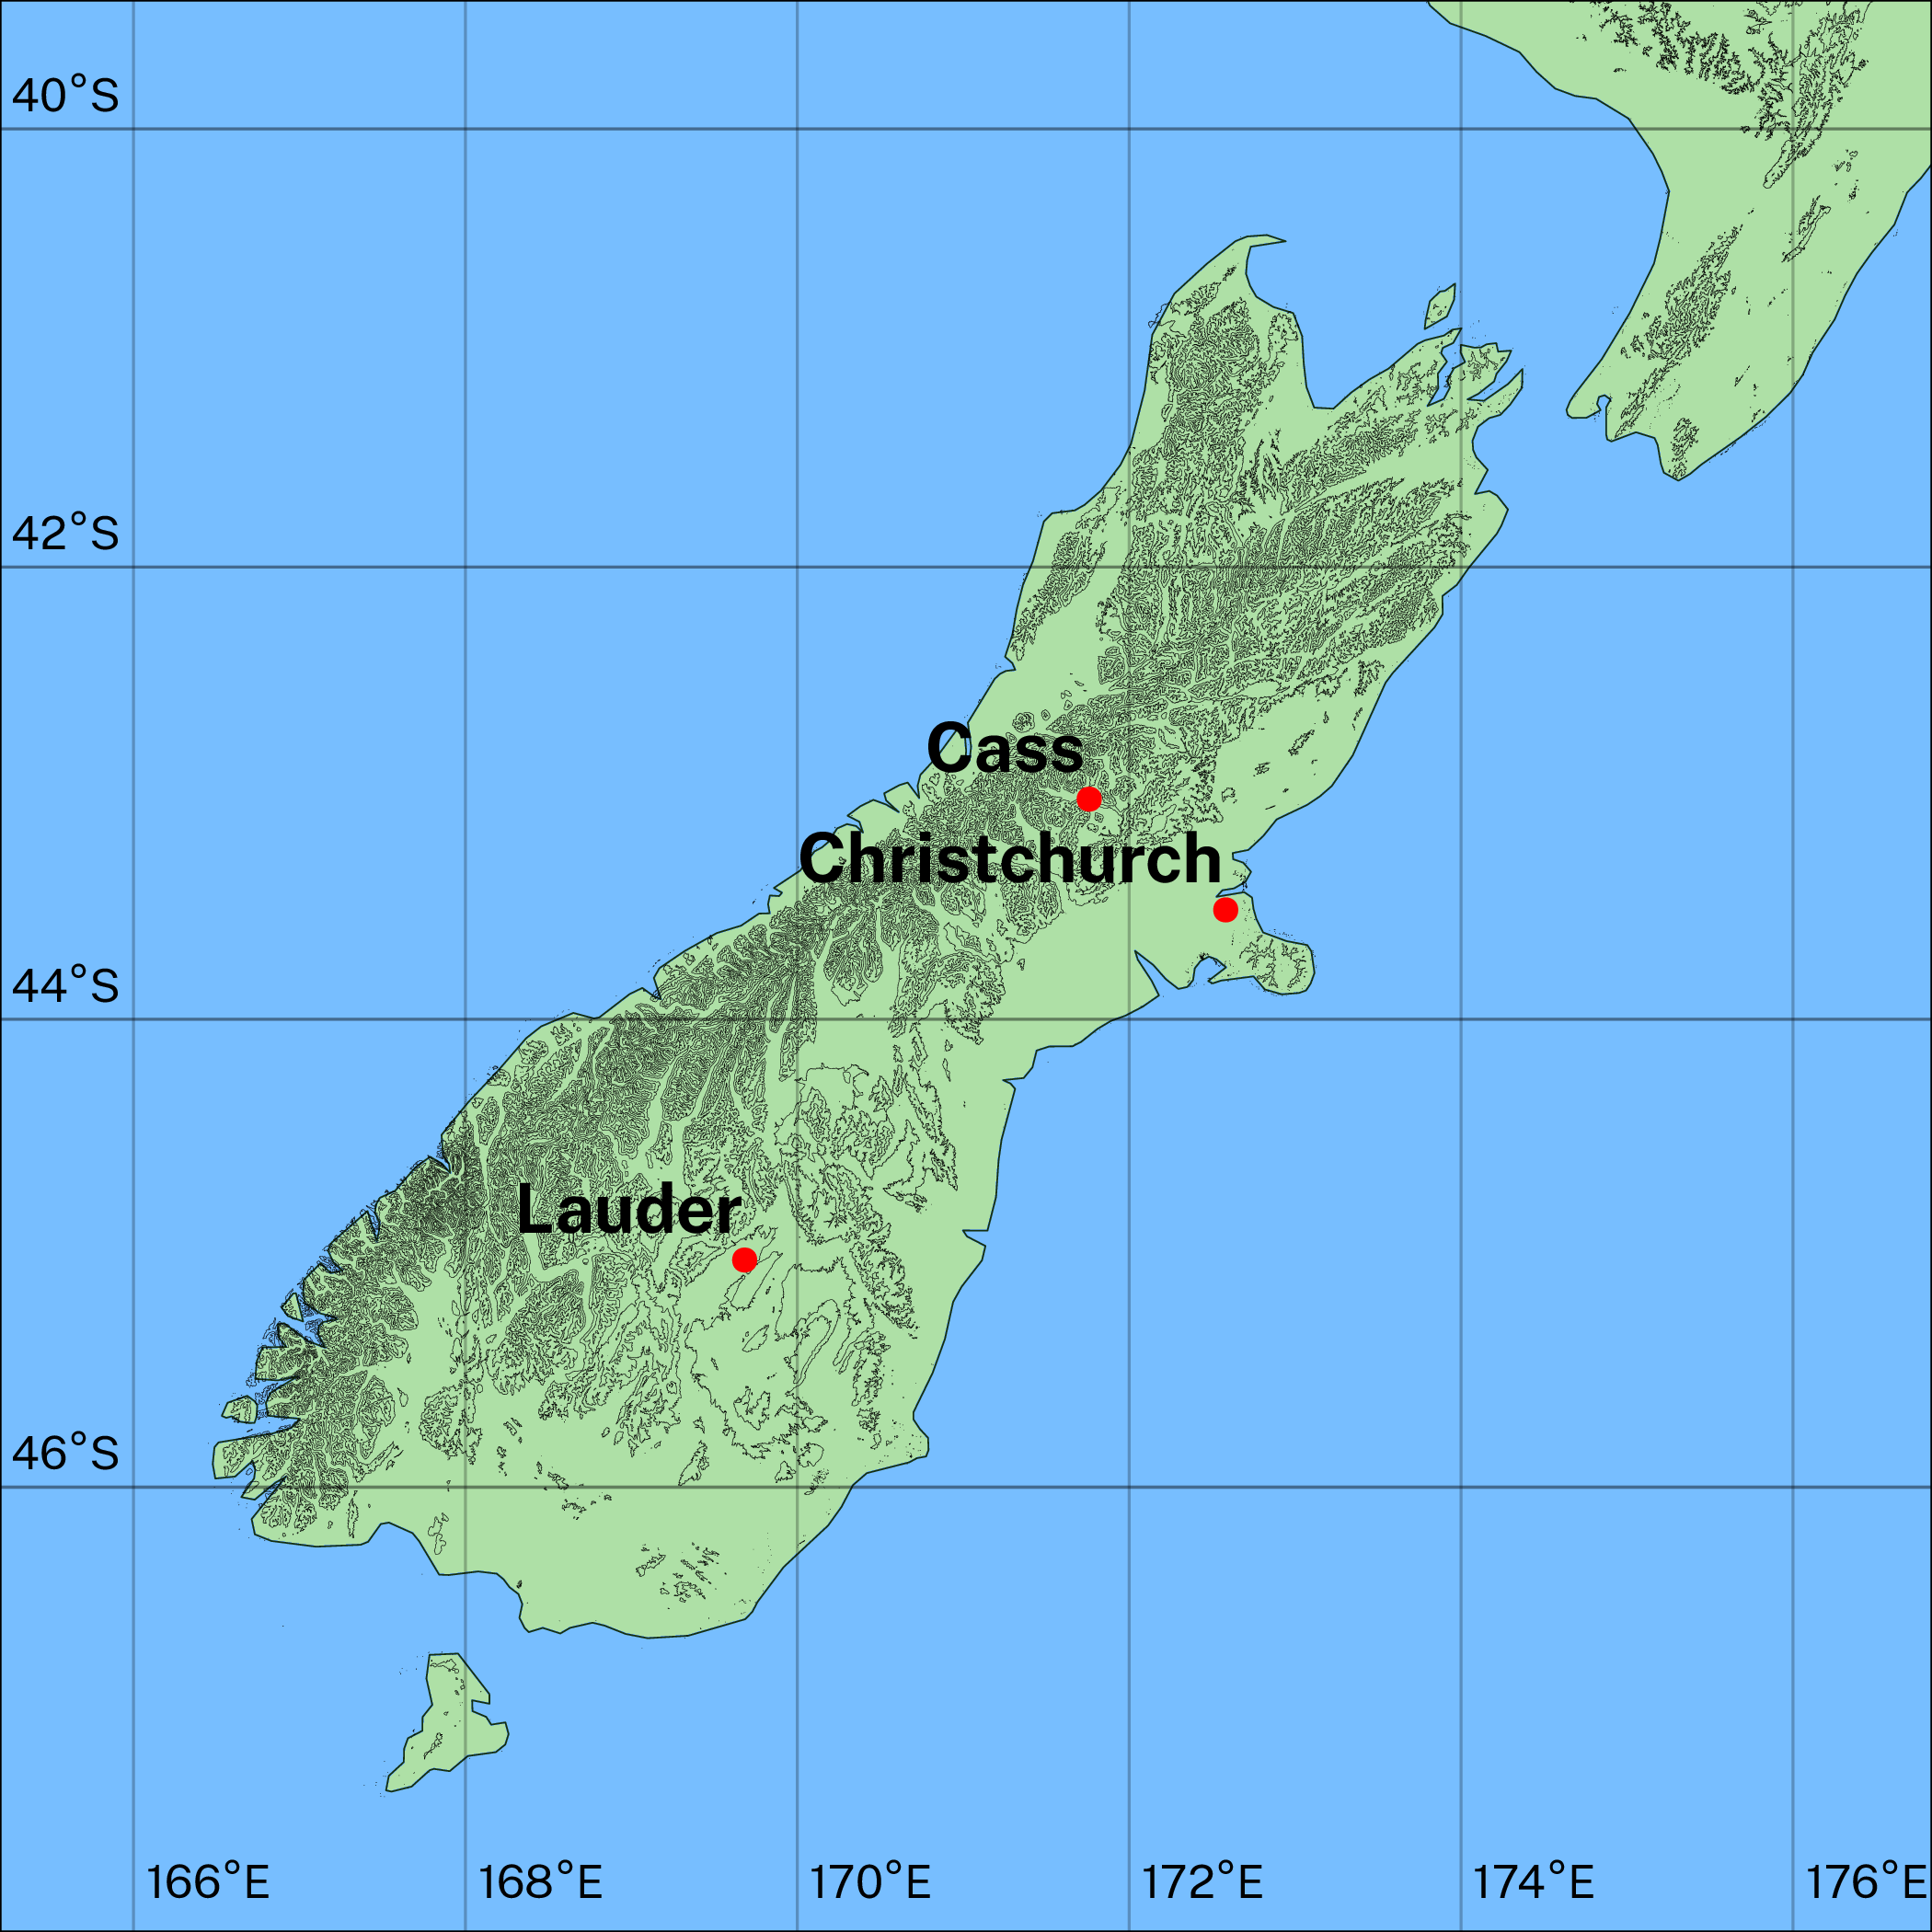
\includegraphics[width=0.6\textwidth]{chapter3/fig/map.png}
\caption[Map showing the location of sites]{Map showing the location of sites. Data at three sites in New Zealand
were analysed: Cass, Lauder and Christchurch.}
\label{fig:3:map}
\end{figure}

\section{Description of case studies}
\label{sec:3:case-studies}

The case studies analysed here were selected
to include all instruments supported by the framework. We compare four different
instruments (CHM 15k, CL31, CL51, MiniMPL) deployed at three locations in NZ
(Lauder, Christchurch, Cass) with three reanalyses (MERRA-2, ERA5, JRA-55),
one NWP model (AMPS) and one GCM (UM).
These case studies aim to demonstrate capability rather than to comprehensively evaluate cloud simulation in the
models and reanalyses. The work detailed in \cite{kuma2020a} provides a detailed evaluation of the UM and MERRA-2 relative to shipborne ceilometer observations.
Figure \ref{fig:3:map} shows the location of the sites and Table \ref{tab:3:case-studies}
summarises the case studies, which are also described in greater detail below.
The sites were chosen from available datasets to demonstrate the use of the
framework with all supported instruments. Two of the sites also had co-located
instruments: CL31 and MiniMPL in Lauder, and CHM 15k and MiniMPL in
Christchurch. The MiniMPL in Lauder and Christchurch were two different units.

\begin{table}[t]
\caption[Location of sites and instruments]{Location of sites and instruments. The time periods are inclusive.}
\label{tab:3:case-studies}
\centering
\scalebox{0.7}{
\begin{tabular}{llllllllll}
\hline
Site & Coordinates & Surface altitude (m) & Instruments & Time period & Missing period & Days\\
\hline
Cass & 43.0346$^\circ$S 171.7594$^\circ$E & 577 & CL51 & 19 Sep--1 Oct 2014 & & 13\\
Lauder & 45.0379$^\circ$S 169.6831$^\circ$E & 370 & MiniMPL, CL31 & 12--24 Jan 2018 & & 13\\
Christchurch & 43.5225$^\circ$S 172.5841$^\circ$E & 45 & MiniMPL, CHM 15k & 17 July--19 August 2019 & 22--31 July & 24\\
\hline
\end{tabular}
}
\end{table}

Cass is a field station of the University of Canterbury
located at an altitude of 577 m in the Southern Alps
of the South Island of NZ. The station is located far from any 
settlements and likely affected little by anthropogenic aerosol relative to the
other sites. We have analysed
13 days of observations with a CL51 at this station performed in September
and October 2014.

Lauder is a field station of NIWA located
inland in the Central Otago region on the South Island of NZ.
The station is situated in a rural area relatively far from large human
settlements. We have analysed 13 days of co-located MiniMPL and CL31
observations made in January 2018. The MiniMPL was operated in a fixed
vertical scanning mode during this period (elevation angle 90\unit{^\circ}).

Observations at the Christchurch site were performed at the
University of Canterbury campus on the Ernest Rutherford building rooftop.
Christchurch is located on the east coast of the South Island of NZ.
Its climate is affected by the ocean, its proximity to the hilly area
of the Banks Peninsula, the Canterbury Plains and föhn-type winds (Canterbury northwester)
resulting from its position on the lee side of the Southern Alps. The city is affected by
significant wintertime air pollution from domestic wood burning and transport.
The orography of the city and the adjacent Canterbury Plains is very flat,
making it prone to inversions. The Ernest Rutherford building is a 5 floor
building situated in an urban area, surrounded by multiple buildings of similar
height. We have analysed 24 days of co-located MiniMPL and CHM 15k observations
performed in July and August 2019. The MiniMPL was operated in a fixed vertical
scanning mode (elevation angle 90\unit{^\circ}).
The nudged run of the UM was only available up to year 2018. Therefore,
it was not analysed for this site.

\begin{figure}[p]
\centering
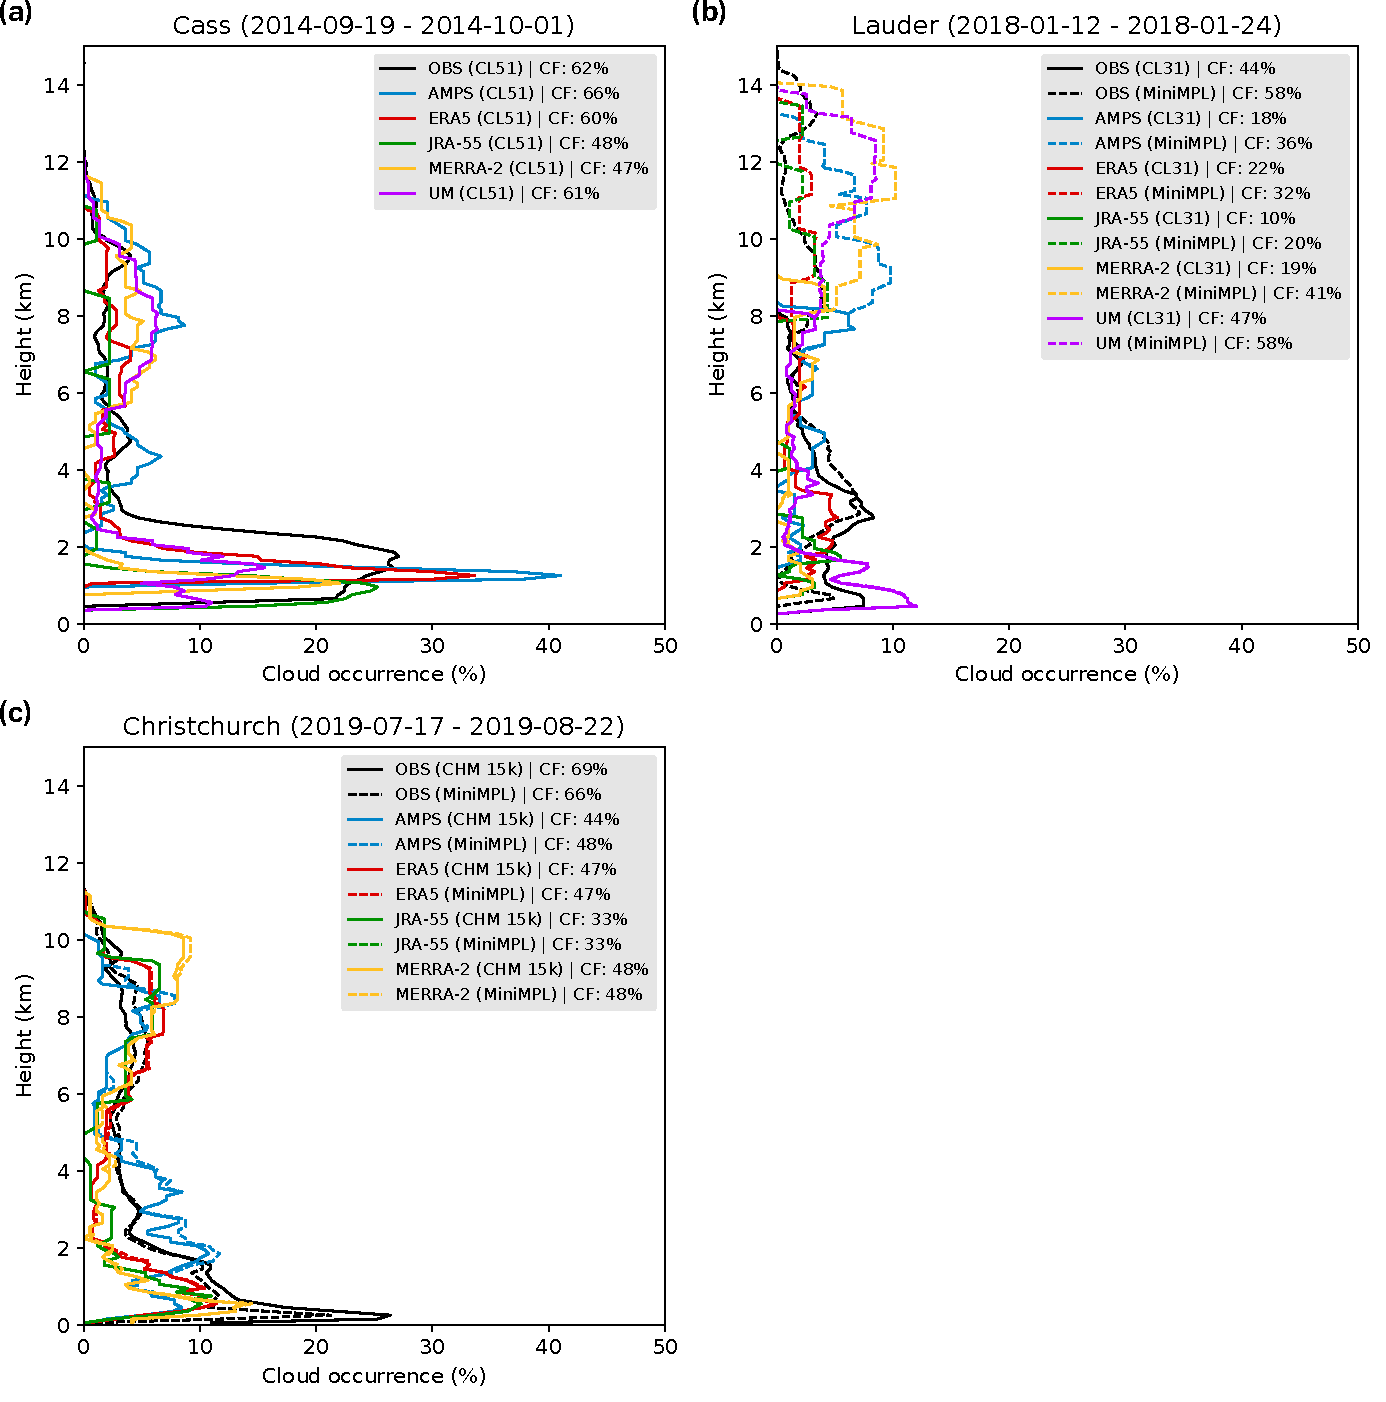
\includegraphics[width=\textwidth]{chapter3/fig/case_studies.pdf}
\caption[Cloud occurrence histogram as a function of height]{
Cloud occurrence histogram as a function of height above the mean sea level
observed at three sites and simulated by the lidar simulator based on atmospheric
fields for five reanalyses and models. Shown is also the total cloud fraction (CF).
The histogram is calculated from the cloud mask as determined by the cloud
detection algorithm.
}
\label{fig:3:case-studies}
\end{figure}

\begin{figure}[p]
\centering
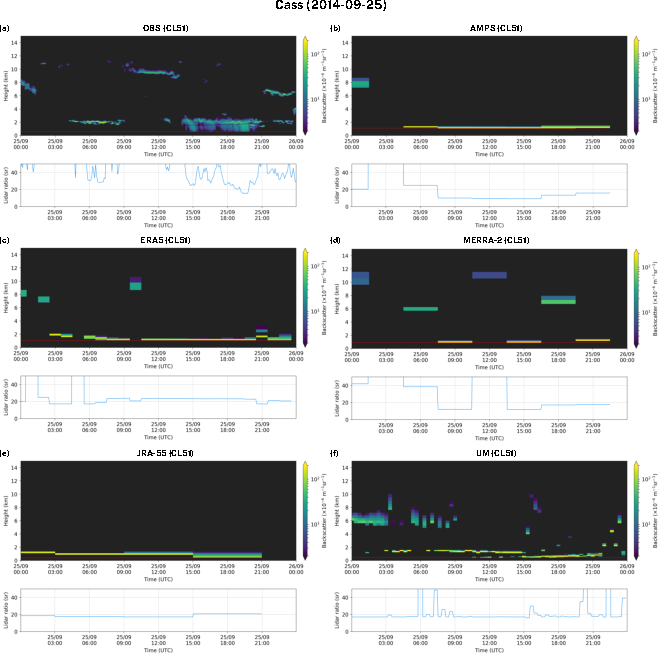
\includegraphics[width=\textwidth]{chapter3/fig/examples.pdf}
\caption[Examples of observed and simulated backscatter profiles]{
Examples of observed (OBS) and simulated backscatter profiles during 24 hours
taken from the three case studies presented here. The observed backscatter
was normalised to absolute units and denoised.
The vertical levels were interpolated based on the
nearest neighbour assumption. The cloud detection threshold of 2\unit{\times 10^{-6} m^{-1}sr^{-1}}
corresponds the low end of the colour scale, i.e. all visible backscatter
in the plots was determined as cloud, unless the difference from the threshold
was smaller than three noise standard deviations. The first subcolumn of
10 columns generated by the Subgrid Cloud Overlap Profile Sampler (SCOPS)
was selected to make the plots. The red line signifies the station altitude.
}
\label{fig:3:examples}
\end{figure}

\begin{figure}[p]
\centering
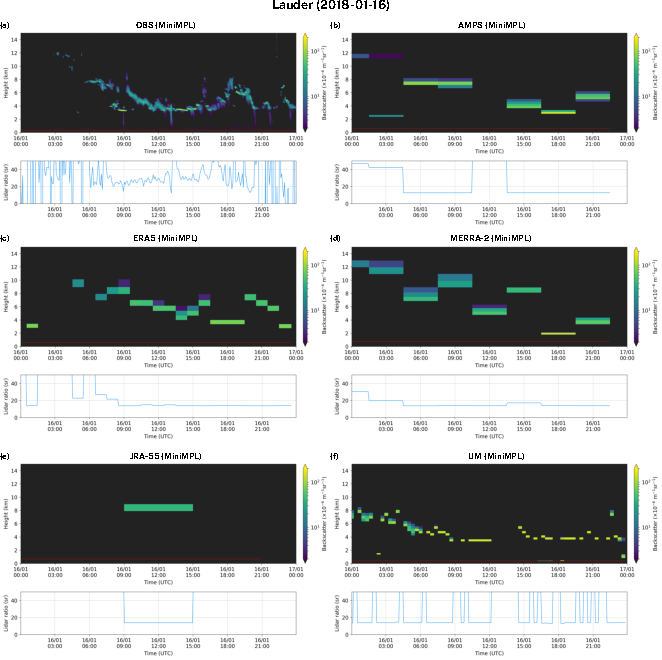
\includegraphics[width=\textwidth]{chapter3/fig/examples2.pdf}
\caption{
The same as Fig. \ref{fig:3:examples} but for the Lauder site.
}
\label{fig:3:examples2}
\end{figure}

\begin{figure}[p]
\centering
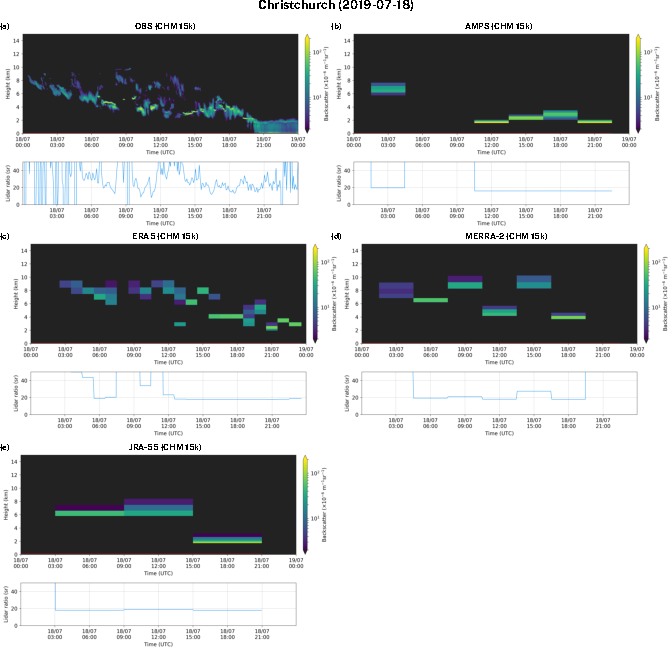
\includegraphics[width=\textwidth]{chapter3/fig/examples3.pdf}
\caption{
The same as Fig. \ref{fig:3:examples} but for the Christchurch site.
}
\label{fig:3:examples3}
\end{figure}

\section{Case study results}
\label{sec:3:results}

To demonstrate the ways that the ALCF can be used we compared a total of 50 days of ALC observations with simulated lidar
backscatter at three sites in NZ (Sect. \ref{sec:3:case-studies}).
The observed backscatter was normalised to calibrated absolute range-corrected
total volume backscattering coefficient. The noise mean as determined at the
furthest range was removed from the backscatter. Cloud detection based on an
attenuated absolute backscatter coefficient threshold of 2 \unit{\times 10^{-6} m^{-1}sr^{-2}}
and three noise standard deviations was applied
to derive a cloud mask and CBH. We compare the statistical cloud occurrence
as a function of height above the mean sea level (ASL) (Fig.
\ref{fig:3:case-studies}) and individual backscatter profiles (selected
profiles are shown in Fig. \ref{fig:3:examples}, \ref{fig:3:examples2} and \ref{fig:3:examples3}) in this section.

We analysed 13 days of CL51 observations at the Cass field station in late
winter. Due to the location of the station at a relatively high altitude in a
varied terrain of the Southern Alps, the models with their
relatively coarse horizontal grid resolution do not represent the
terrain and position accurately. The orography representation of the models meant
that the virtual altitude of the station was 1115 m (AMPS), 1051 m (ERA5),
401 m (JRA-55), 914 m (MERRA-2) and  428 m (UM). The virtual position, which is the centre
of the nearest model grid cell to the site location, ranged from relatively
close in the Southern Alps (AMPS, ERA5, MERRA-2, UM) to relatively far on the West
Coast of NZ (JRA-55) depending on the horizontal resolution of the grid. The time period examined was characterised by diverse cloud
occurrence with periods of low cloud and precipitation, mid-level cloud,
fog, high cloud and clear skies. Precipitation, currently not simulated by the
lidar simulator, was present in about 18\% of the observed backscatter profiles,
as determined by visual inspection.
Figure \ref{fig:3:case-studies}a shows that predominantly low cloud and
precipitation between the ground and 2 km ASL in 25\% of
profiles was observed. Cloud between 3 and 12 km ASL was observed about
evenly in 2\% of profiles. While the reanalyses and models were able to partially
reproduce the peak of cloud occurrence near 1 km ASL, the peak they displayed is less vertically broad than observed,
and in the UM the peak was much weaker than observed.
The lack of precipitation simulation
might also have contributed to this apparent difference between observed and simulated
cloud. Above 3 km ASL, the reanalyses and models tended to overestimate cloud,
with only ERA5 and JRA-55 simulating close to the observed cloud occurrence.
The observed total CF was 62\%. AMPS overestimated this value by 4 percentage points (pp),
ERA5 and the UM reproduced almost the exact value (within 2 pp), while the other reanalyses (JRA-55 and MERRA-2)
underestimated CF by about 15 pp.

We also analysed 13 days of CL31 and MiniMPL observations at the Lauder station
in summer. During the time period relatively diverse cloud was observed,
with periods of low, mid- and high cloud, clear sky and a small fraction
of profiles with precipitation (about 3\%). The altitude of the station of 370 m
ASL generally had a much higher equivalent in the reanalyses and models:
565 m (AMPS), 642 m (ERA5), 681 m (JRA-55) and 786 m (MERRA-2) due to the
presence of hills in the surrounding region (the station is in a high valley),
with the exception of the UM where the altitude was 385 m. The virtual station position in the
reanalyses and models ranged from relatively close to the station in the same
geographical region (AMPS, ERA5), a nearby location in a more hilly region
(JRA-55), a relatively distant location in the adjacent Dunstan Mountains
(MERRA-2) and a relatively distant location in Central Otago (UM).
Figure \ref{fig:3:case-studies}b shows that the CL31 observed relatively even cloud occurrence between the ground
and 3 km ASL at 8\%, falling off to about 3\% between 4 and 8 km ASL
(the maximum lidar range of CL31 is 7.7 km). The MiniMPL observed much weaker
backscatter than CL31 below 3 km ASL, which was identified as an overlap
calibration issue in the MiniMPL.
The MiniMPL observed
substantial amounts of cloud above 8 km, not present in the CL31 observations
due to its range limitation. Overall, the observed cloud occurrence had two
peaks at ground to 3 km ASL and at about 9 km ASL. The simulated cloud
occurrence was generally underestimated between the ground and 5 km ASL,
with the exception of the UM which reproduced the lower half of the peak
accurately, and ERA5 which reproduced the upper half of the peak accurately.
Above 5 km ASL, the cloud occurrence was well reproduced in ERA5 and JRA-55,
and strongly overestimated in AMPS, MERRA-2 and the UM. The reanalyses and models also
tended to have two peaks at about 2 km ASL and 11 km ASL, but these were quite
different from the observed peaks, with the lower peak underestimated by about
5 pp in the reanalyses and models and the higher peak overestimated by about 5--10 pp.
The total CF was observed as 44\% and 58\% by CL31 and MiniMPL, respectively.
CF observed by the MiniMPL was likely higher due to its higher maximum lidar range
(CL31 missed a substantial amounts of high cloud due to this limitation).
The total CF was strongly underestimated by the reanalyses and models
by up to 34 pp (CL31) and 38 pp (MiniMPL), with the exception of the UM
which simulated the correct CF within 3 pp.

The Christchurch observations were taken during a total of 24 days in mid-
to late winter. The cloud situations were characterised by the frequent occurrence of low cloud
and fog, with relatively diverse mid- and high level cloud and periods of clear
sky also present (not shown). Precipitation was present in about 9\% of profiles and fog
in about 11\% of profiles. As the site location is relatively flat
(Canterbury Plains), the models didn't have any difficulty in reproducing the
altitude of the site, which was 32 m (AMPS), 72 m (ERA5), 143 m (JRA-55) and
76 m (MERRA-2). The virtual location was within the boundaries of the city
(AMPS), on the Canterbury Plains close to the city boundaries (ERA5, MERRA-2),
and over Lake Ellesmere about 20 km from the city (JRA-55).
Figure \ref{fig:3:case-studies}c shows that the co-located CHM 15k and MiniMPL
observed a strong peak of cloud occurrence of 26\% (CHM 15k) and 20\% (MiniMPL) at about 500 m ASL. This was
likely due to the combined precipitation and fog as well as false detection
of aerosol as cloud. The observed cloud occurrence
had a local minimum of 2\% at about 5 km ASL, a secondary peak of
5\% at 7 km ASL, and fell off 0\% at 11 km ASL.
The CHM 15k and MiniMPL observations showed inconsistencies
of up to 5 pp. The reanalyses and
models strongly underestimated low cloud by about 10-20 pp. With the
exception of AMPS, they underestimated mid-level cloud by about 5 pp and
represented high cloud relatively accurately.
The total CF observed was 69\% and 66\% for the
CHM 15k and MiniMPL, respectively, while the reanalyses and models strongly
underestimated CF by up to 36 pp (JRA-55), with
underestimates around 20 pp common.

Figures \ref{fig:3:examples}, \ref{fig:3:examples2}, \ref{fig:3:examples3} show images of backscatter for three separate days taken from
the three case studies. The selected days represent some of the best-matching
profiles and demonstrate how well the reanalyses and models can simulate cloud under
favourable conditions. As can be seen in the figures, 
the UM performs the best
in terms of temporal and height accuracy of the simulated cloud
(Fig. \ref{fig:3:examples}f, \ref{fig:3:examples2}f), followed by ERA5
(Fig. \ref{fig:3:examples}c, \ref{fig:3:examples2}c, \ref{fig:3:examples3}c). This is likely
due to the high output temporal resolution of the UM and ERA5 of 20 min. and 1 h,
respectively.
The UM and ERA5 were able to represent the relatively fine structure of cloud and to a lesser extent
the optical thickness (inferred from the strength of backscattering) of the cloud.
Deficiencies, however, are readily
identifiable.
The low cloud in the UM (Fig. \ref{fig:3:examples}f) appears to be shifted by several
hours relative to observations (Fig. \ref{fig:3:examples}a) and the high cloud
has a greater vertical extent in the UM. Likewise, the altocumulus cloud
observed in Fig. \ref{fig:3:examples2}a is shifted by several hours in the UM
(Fig. \ref{fig:3:examples2}f). The stratocumulus and nimbostratus cloud, identified visually based on the backscatter profiles, in ERA5 (Fig. \ref{fig:3:examples}c)
is markedly lower than observed (Fig. \ref{fig:3:examples}a),
as well as optically thicker than in reality.
The mid-level cloud in ERA5 (Fig. \ref{fig:3:examples2}c) was located about 2 km higher than observed (Fig. \ref{fig:3:examples2}a).
Precipitation observed in Fig. \ref{fig:3:examples3}a towards the end of the analysed period was not present in the ERA5
simulated profile (Fig. \ref{fig:3:examples3}c) due to lack of precipitation simulation
in the current lidar simulator (even though rain and show specific content is available from the reanalysis).
MERRA-2 was the third-best performing
reanalysis in terms of cloud representation accuracy. The reanalysis managed
to capture the overall structure of clouds (Fig. \ref{fig:3:examples}c, g, k),
but substantial discrepancies were present, some of which were likely due to the
relatively low temporal resolution of the reanalysis (3 h). AMPS was
identified as the fourth-best in terms of cloud representation accuracy despite the highest spatial resolution of the model. Fig.
\ref{fig:3:examples}h shows that while the overall structure of the cloud is
represented in the reanalysis, it was not able to represent any of the finer
details. This is likely partially due to the temporal resolution of the model output of just 3 h
(AMPS has, however, relatively high horizontal grid resolution of 21 km).
 A visual comparison of AMPS and MERRA-2 with observations suggests that the
the MERRA-2 simulations are more accurate than AMPS despite the
fact that the horizontal grid resolution of AMPS is much finer than MERRA-2.
This demonstrates that other factors in the model than resolution have
stronger influence on the quality of cloud simulation.
JRA-55
was identified as the last in terms of cloud representation accuracy. JRA-55
has the lowest temporal resolution of the studied reanalyses and models of
just 6 h, as well as the lowest horizontal grid resolution of 139 km. Therefore,
it cannot be expected to capture any fine details of cloud. In the presented
profiles (Fig. \ref{fig:3:examples}d, l) one can see that the cloud is only
crudely represented. JRA-55 was able to represent the stratocumulus cloud
of Fig. \ref{fig:3:examples}a, although its temporal extent and optical thickness
were overestimated. The mid-level cloud of Fig. \ref{fig:3:examples}i was
relatively well-represented in terms of height and optical thickness
(Fig. \ref{fig:3:examples}l), given the low temporal resolution of the reanalysis.
We stress that a direct backscatter profile intercomparison is highly dependent
on the temporal resolution of the model output. The statistical intercomparison,
however, should still give unbiased results if the cloud physics is accurately
simulated by the atmospheric model.

\begin{figure}[t]
\centering
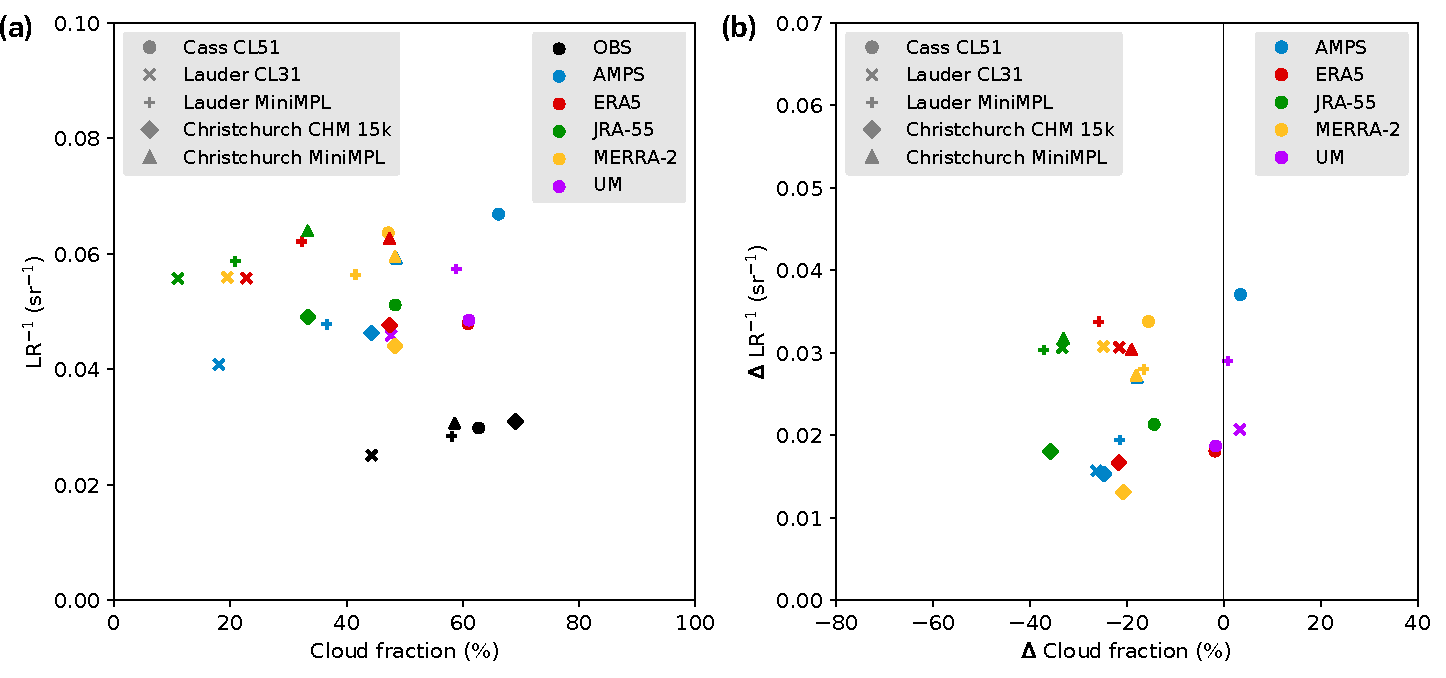
\includegraphics[width=\textwidth]{chapter3/fig/scatter.pdf}
\caption[Scatter plot showing the average cloud fraction and the average inverse lidar ratio]{
\textbf{(a)} Scatter plot showing the average cloud fraction calculated from all profiles
and the average inverse lidar ratio (LR$^{-1}$) calculated from cloudy profiles
for the case studies. The site and instrument are coded by the shape of the
marker and the observation (legend in the top left corner), reanalysis or model
is coded by the colour of the marker (legend in the top right corner).
\textbf{(b)} The same as (a), but showing relative differences between
the reanalyses and models relative to the corresponding observations.
}
\label{fig:3:scatter}
\end{figure}

The comparison between observations, reanalyses and models can be summarised
by considering that the radiative effect of clouds is the product of
cloud occurrence/fraction and their albedo. CF can be derived
from ALC observations by determining the cloud mask and identifying cloudy
profiles which contain detected cloud. Cloud albedo cannot be
directly observed with ALCs due to the unknown backscatter-to-extinction ratio of
the cloud layers, which depends on the cloud phase, the effective radius
and the shape of ice crystals. However, we can use LR, calculated from
the vertically integrated backscatter, as a proxy for cloud albedo. Clouds which
are not fully opaque result in LR which is greater than the expected theoretical
LR based on the Mie theory (Fig. \ref{fig:3:size-dist}). The inverse of LR (extinction-to-backscatter ratio)
is therefore approximately proportional to the albedo of the cloud.
Figure \ref{fig:3:scatter}a, b shows an absolute and relative (respectively) scatter plot of the average cloud fraction
and the average of the inverse of LR calculated from cloudy profiles.
As already shown in Fig. \ref{fig:3:case-studies}, the reanalyses and models generally underestimate
CF. However, Fig. \ref{fig:3:scatter} shows that this is compensated by overestimated albedo (higher LR$^{-1}$
indicates higher cloud albedo), which is higher in all reanalyses and models
than the corresponding ALC observations. Further examination shows that the UM and ERA5 show the closest
proximity to the corresponding observations in terms of the average CF and LR$^{-1}$. The Lauder CL31 and MiniMPL
also show a stark difference in CF, with the CL31 detecting much smaller CF due
to its maximum vertical range limitation of 7.7 km, which causes a significant
fraction of high cloud to be omitted. The results shown in Fig. \ref{fig:3:scatter}
suggest that the "too few too bright" model cloud problem identified in
previous studies \citep{nam2012,klein2013,wall2017,kuma2020a} is also observed in the current case studies, whereby the
simulated CF is too low, but its exaggerated albedo means that
the top of the atmosphere (TOA) shortwave radiative balance can be approximately
correct.

\begin{figure}[p]
\centering
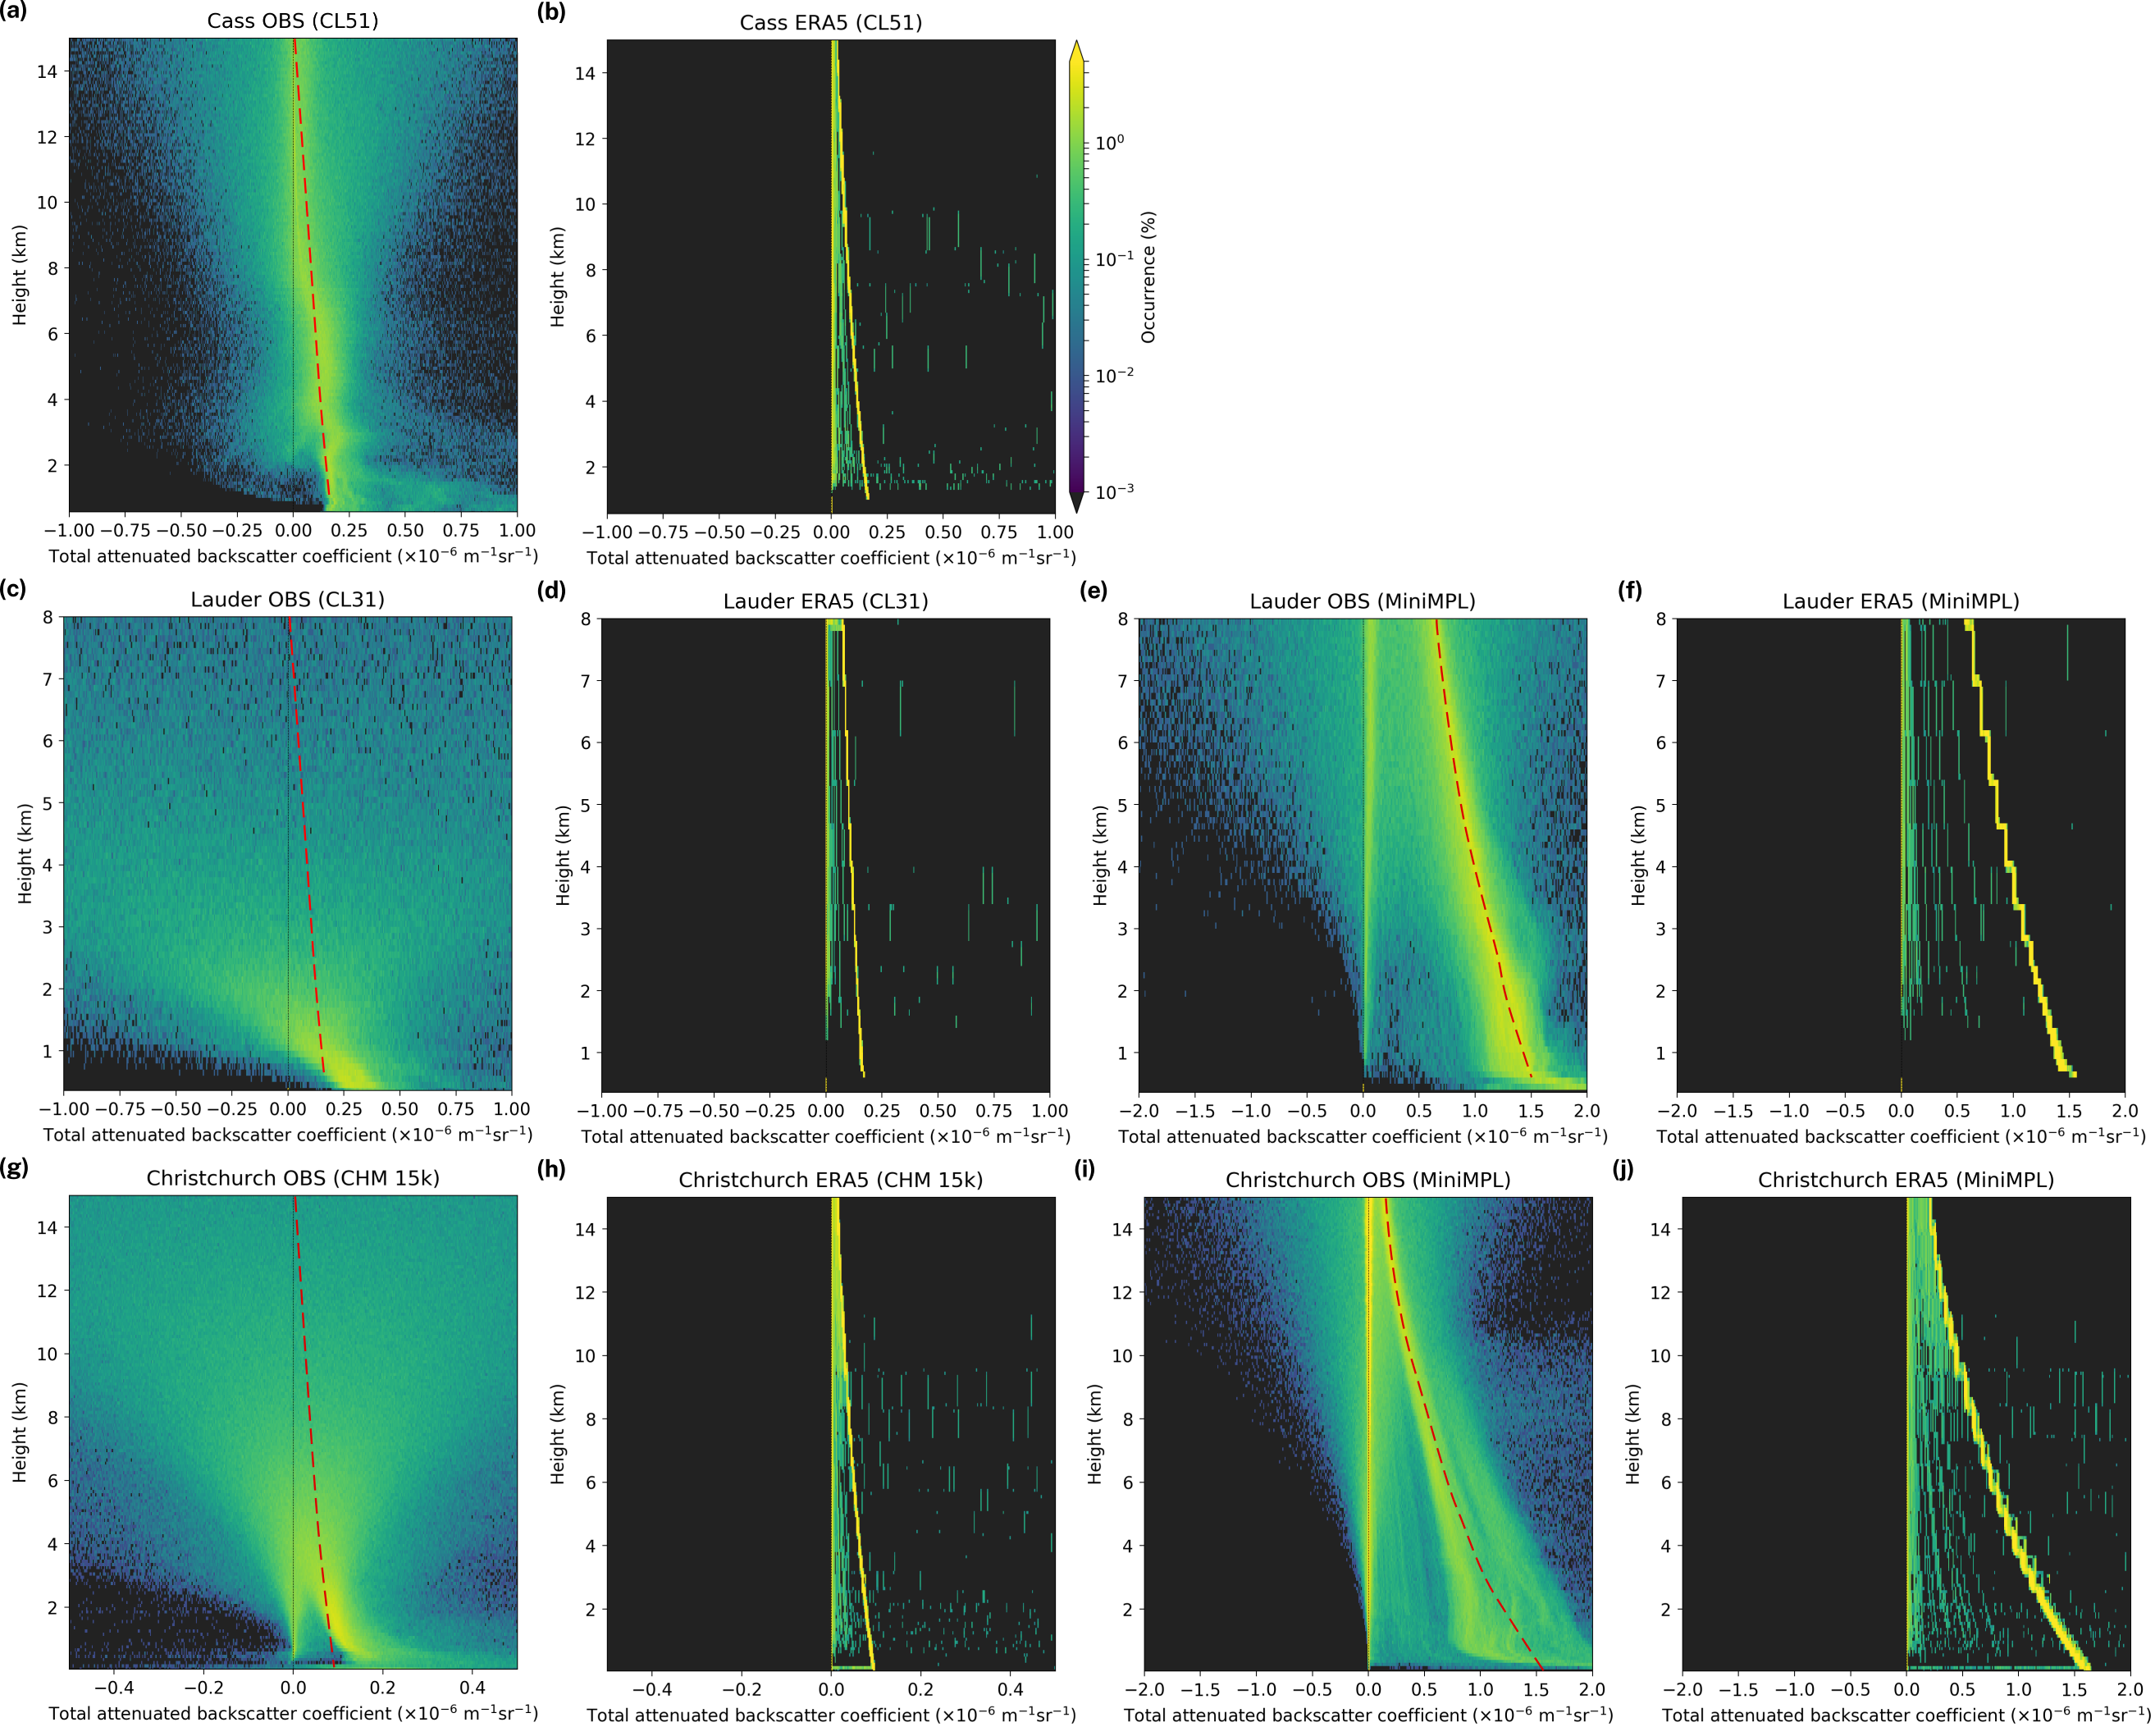
\includegraphics[width=\textwidth]{chapter3/fig/backscatter_hist_micro.png}
\caption[Backscatter histograms as a function of height]{
Backscatter histograms as a function of height observed and simulated
at three different sites of the case studies calculated from all profiles.
The plots show the distribution
of backscatter for values which are on the scale of noise, molecular and
aerosol backscatter ([-0.5, 0.5] for CHM 15k, [-1, 1] for CL31 and CL51 and 
[-2, 2] \unit{\times 10^{-6}m^{-1}sr^{-1}} for MiniMPL).
The simulated backscatter is based on the ERA5
atmospheric fields. Visible in the plots is backscatter caused by molecular
backscatter (the main "streak"), noise when signal is fully attenuated by cloud
(the zero-centred "streak"), and the range-dependent noise
(the zero-centred "cone"). The molecular backscatter is marked by a red dashed
line on the observed backscatter plots, the shape of which is taken from
the simulated molecular backscatter for the corresponding instrument and site.
}
\label{fig:3:micro-backscatter}
\end{figure}

\begin{figure}[p]
\centering
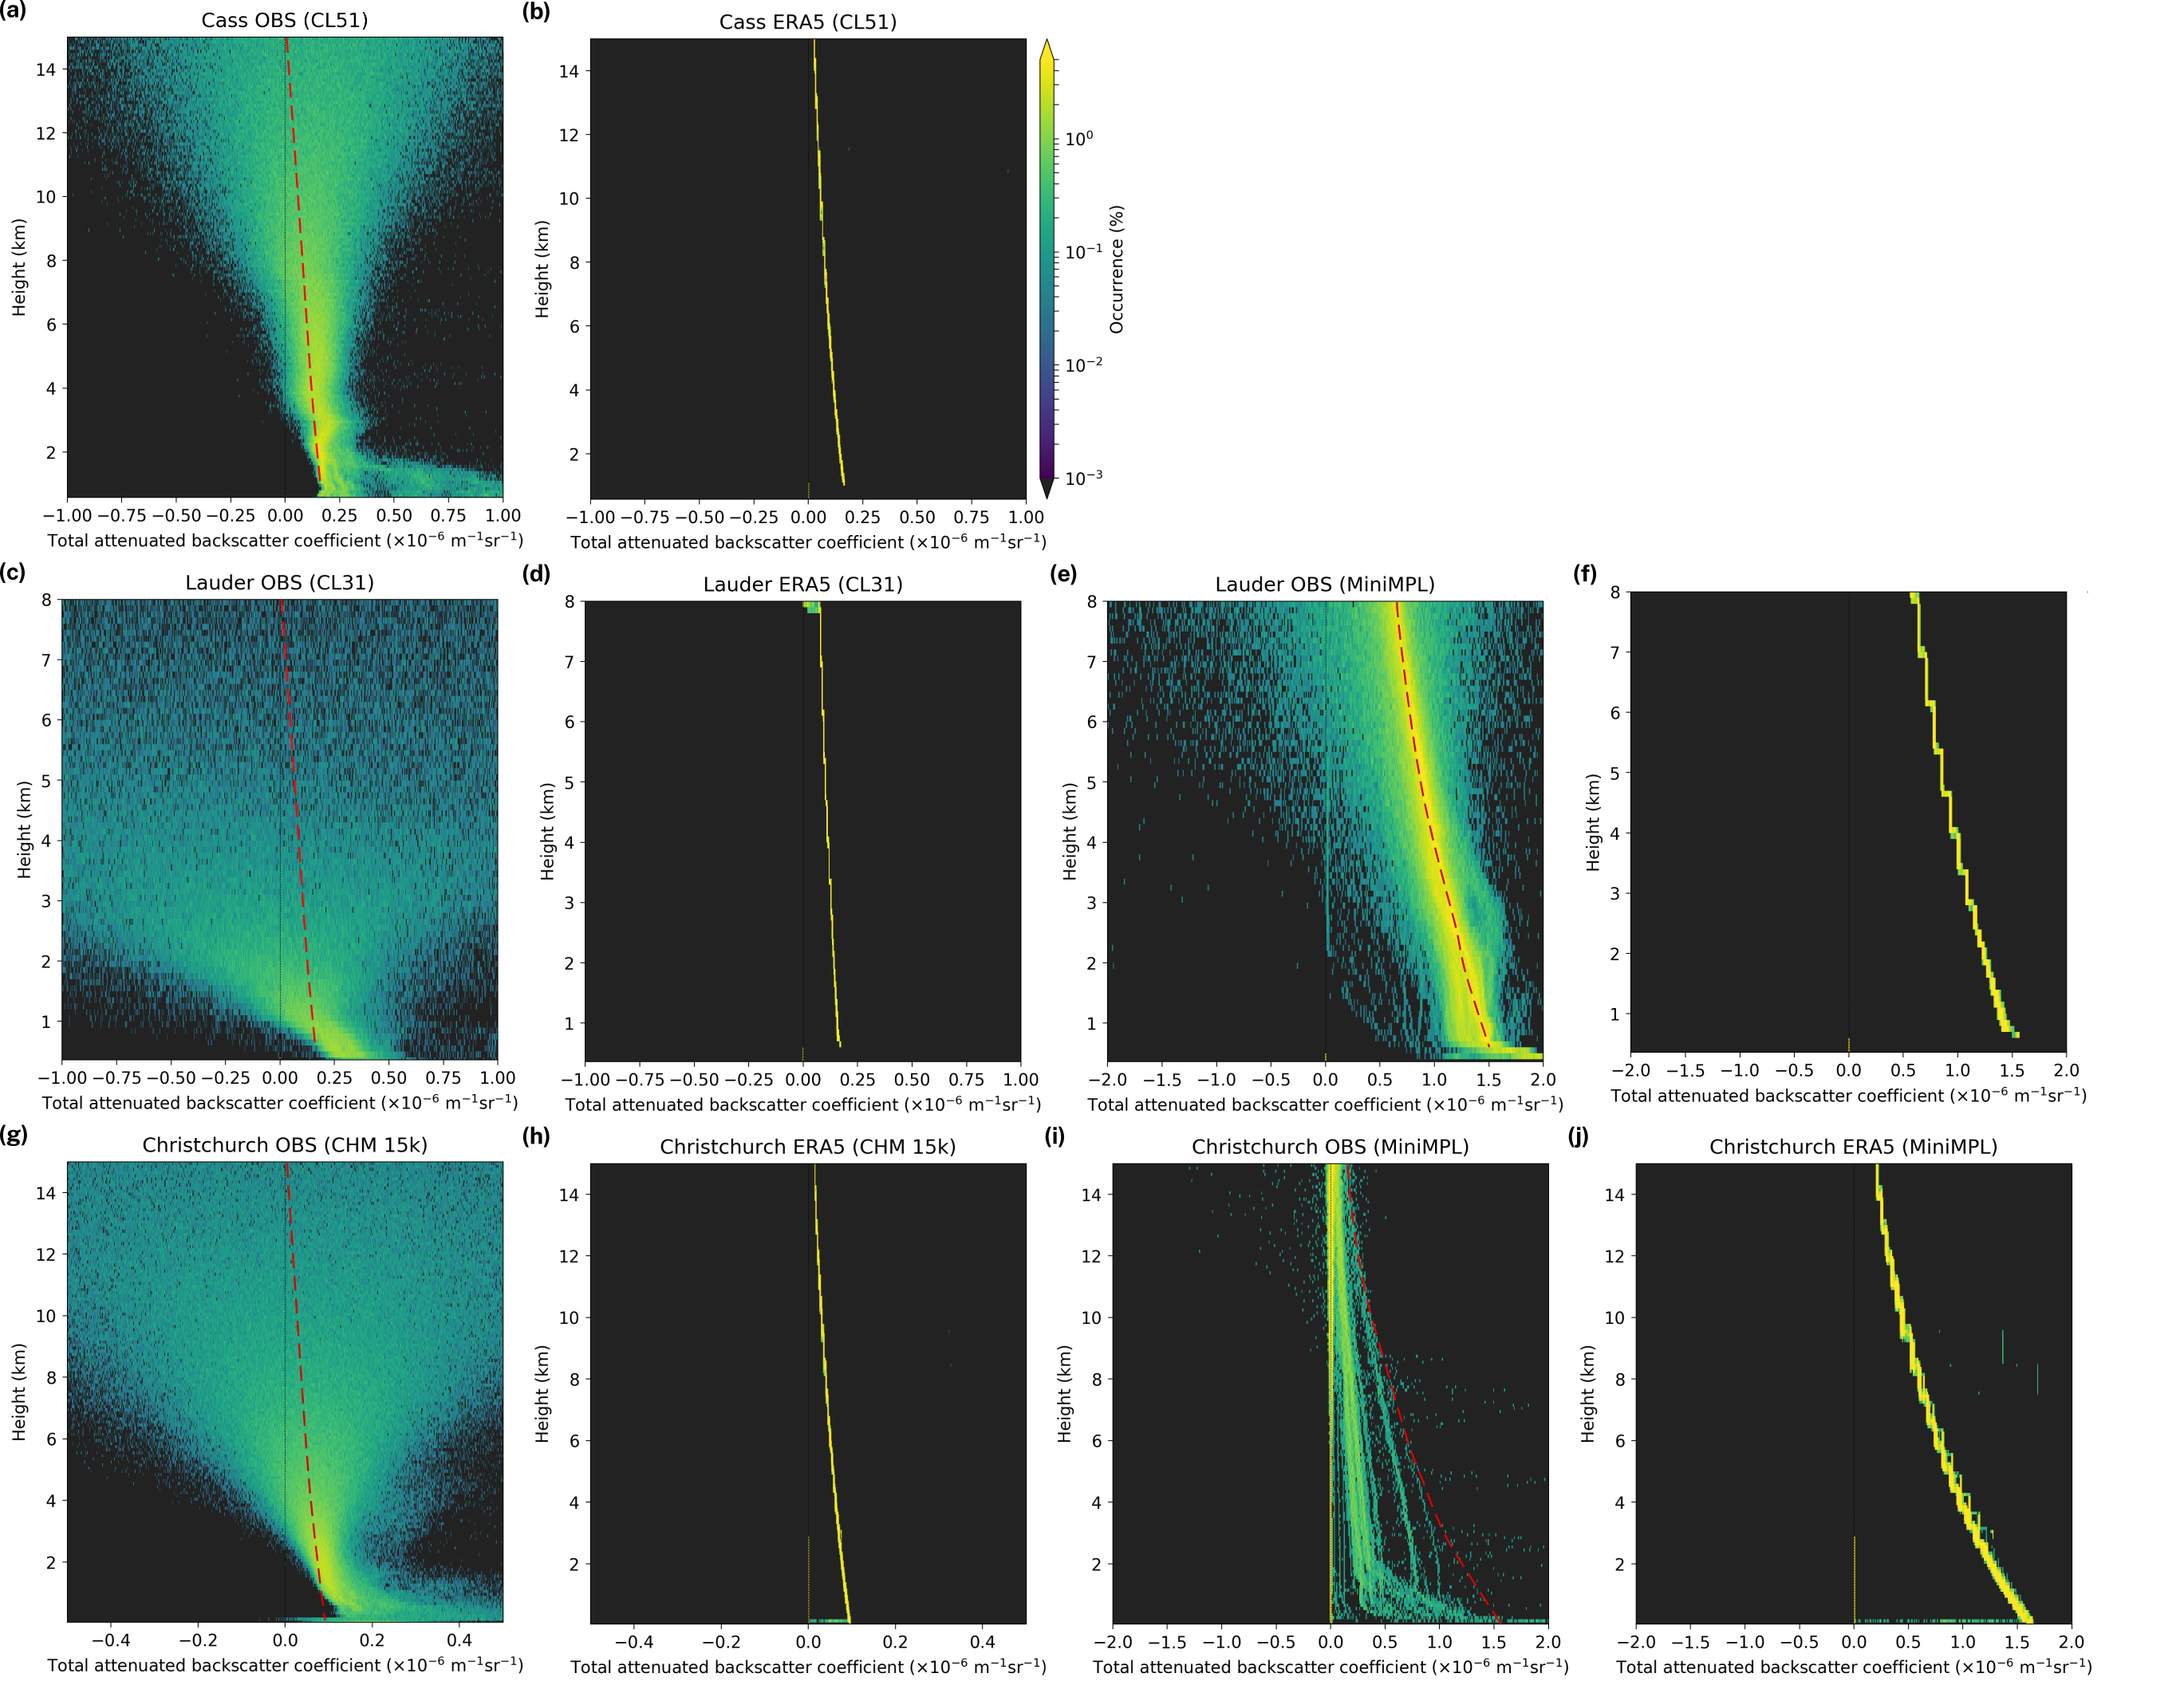
\includegraphics[width=\textwidth]{chapter3/fig/backscatter_hist_micro_clear.png}
\caption{
The same as Fig. \ref{fig:3:micro-backscatter} but calculated from clear
sky profiles only.
}
\label{fig:3:micro-backscatter-clear}
\end{figure}

Figure \ref{fig:3:micro-backscatter} shows backscatter histograms as a function of
height for small values of backscatter (up to 2\unit{\times 10^{-6}m^{-1}sr^{-1}})
observed and simulated at the sites of the case studies, calculated for
the entire time period of each case study. The scale of values is below
cloud backscatter, and therefore shows backscatter which results from molecular and
aerosol scattering and noise. Molecular backscattering depends on the
atmospheric pressure and temperature as well as the lidar wavelength.
It causes the main "streak" (a local maximum) visible in each of the histograms. The observed molecular
backscattering value at the surface approximately corresponds to the
theoretically calculated value at each wavelength: 0.0906 \unit{\times 10^{-6}m^{-1}sr^{-1}} ($\lambda$ = 1064 nm),
0.172 \unit{\times 10^{-6}m^{-1}sr^{-1}} ($\lambda$ = 910 nm) and 1.54 \unit{\times 10^{-6}m^{-1}sr^{-1}} ($\lambda$ = 532 nm) at 1000 hPa and 20\unit{^\circ C}
(Table \ref{tab:3:mol-backscatter}). The molecular backscattering in the boundary
layer is, however, superimposed on backscattering by aerosol and cloud. In the case
of the MiniMPL observations at the Christchurch site (Fig. \ref{fig:3:micro-backscatter}i),
the molecular backscatter streak has multiple secondary streaks. These are caused by different levels
of attenuation by cloud and aerosol during the period of the observations.
These secondary streaks were also partially reproduced by the simulator
(Fig. \ref{fig:3:micro-backscatter}j).
A smaller portion of the width of the streak is also caused by fluctuations of atmospheric
temperature and pressure. Under suitable conditions, the molecular backscatter
can be used for absolute calibration of an instrument. With the exception 
of CL31 (Fig. \ref{fig:3:micro-backscatter}c), the molecular backscatter can
be identified in the observed backscatter in each case. Therefore, it is possible to
choose a calibration coefficient such that the observed and simulated
molecular backscatter overlap. This can be considered a viable alternative
to the liquid stratocumulus LR calibration method, or as a means of
cross-validating the instrument calibration. However, it should be noted that the accuracy of this method
is affected by an unknown amount of aerosol attenuation. Cloudy profiles
can be filtered when calculating the histogram, and therefore the effect of
cloud attenuation can be minimised.
In addition to the molecular backscatter streak,
there is a zero-centred streak visible in the histograms. This is caused
by noise when the signal is fully attenuated by cloud. Lastly, a zero-centred
"cone" of noise is visible in the observed backscatter, increasing with the
square of range. The size of this cone is particularly large in the case
of the CL31 (Fig. \ref{fig:3:micro-backscatter}c), which is most likely the result
of its low receiver sensitivity and low power compared to the other
instruments. The standard deviation of the cone at the furthest range
is used to determine the noise standard deviation used by the cloud
detection algorithm (Sect. \ref{sec:3:cloud-detection}).

\begin{figure}[t]
\centering
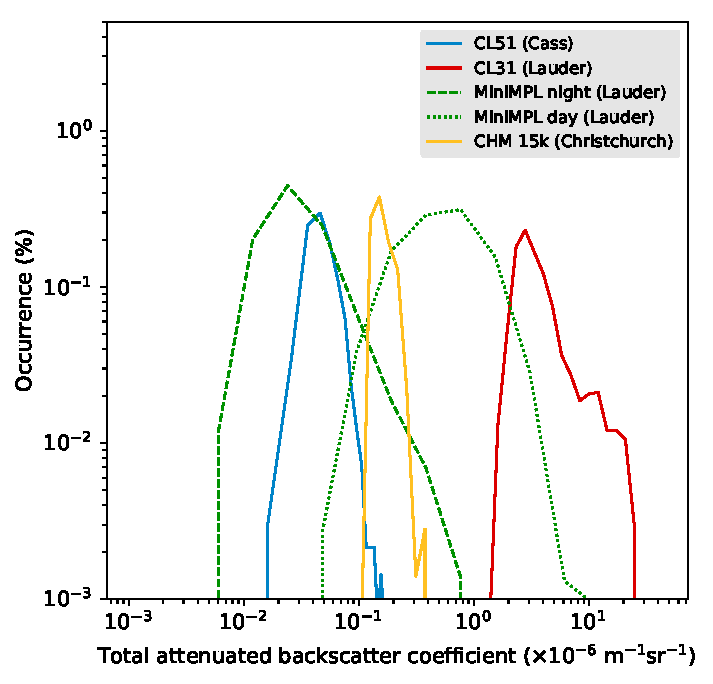
\includegraphics[width=0.6\textwidth]{chapter3/fig/backscatter_sd_hist.pdf}
\caption[Backscatter noise standard deviation histogram]{
Backscatter noise standard deviation histogram calculated for each instrument
at sites of the case studies from clear sky profiles over the whole time period.
The noise distribution is calculated at the furthest range. Shown is the
range-scaled noise distribution at a range of 7 km. The MiniMPL nighttime and daytime
distributions are calculated from nighttime and daytime profiles only, determined
the by position of the Sun below and above the horizon, respectively, at
the geographical position of the site and time when the profile was observed.
}
\label{fig:3:backscatter-sd-hist}
\end{figure}

Figure \ref{fig:3:micro-backscatter-clear} shows the same information as Fig. \ref{fig:3:micro-backscatter},
but for clear sky profiles only. Here, it can be seen that the zero-centred
peak caused by the complete attenuation by cloud is no longer present.
There is a clear overlap between the centre of the noise cone
with the simulated molecular backscatter; i.e. the noise cone is centred
at the observed molecular backscatter. This is visible with all instruments
including CL31 (Fig. \ref{fig:3:micro-backscatter-clear}c), where the overlap between
the observed and simulated molecular backscatter is most clearly visible at about 1 km ASL.
Below 1 km ASL,
the effect of boundary layer aerosol distorts the molecular backscatter
by an unknown quantity. The clear sky histograms as shown in Fig.
\ref{fig:3:micro-backscatter} may therefore be preferable to the all-sky
histograms of Fig. \ref{fig:3:micro-backscatter} for calibration by fitting 
the molecular backscatter. Note that Figure \ref{fig:3:micro-backscatter-clear}i
does not show a good match with the simulated molecular backscatter (Fig. \ref{fig:3:micro-backscatter-clear}j)
likely due to miscalibration of the MiniMPL in the lower troposphere,
which causes spurious cloud to be detected. The majority of profiles were therefore
filtered out as cloudy. The dead time, afterpulse and overlap MiniMPL
calibration supplied by the vendor appears to be deficient and causes
range-dependent bias in the backscatter profile.

We now examine the noise in each instrument using the ALCF.
Figure \ref{fig:3:backscatter-sd-hist} shows the distribution of standard
deviation of backscatter noise determined at the highest observable range of each instrument
and range-scaled
to 7 km. It can be seen that the CL31 is affected by the greatest amount of noise,
peaking at about 2\unit{\times 10^{-6}m^{-1}sr^{-1}}. This is at the
threshold of cloud detection of 2\unit{\times 10^{-6}m^{-1}sr^{-1}}. Therefore,
thin cloud may be obscured by noise at higher ranges with this instrument. The MiniMPL,
operating in the visible spectral range, shows a bimodal distribution of
backscatter noise depending on sunlight. During daytime, it peaks at
about 0.7\unit{\times 10^{-6}m^{-1}sr^{-1}}, which is the second highest
of the analysed instruments. During nighttime, it peaks at about
0.02\unit{\times 10^{-6}m^{-1}sr^{-1}}, which is the lowest of the analysed
instruments. The CHM 15k histogram peaks between the nighttime and daytime MiniMPL at 0.2\unit{\times 10^{-6}m^{-1}sr^{-1}}.
CL51 observed the second lowest amount
of noise after the nighttime MiniMPL at about 0.04\unit{\times 10^{-6}m^{-1}sr^{-1}}.
The difference between nighttime and daytime backscatter noise in the MiniMPL
has been previously analysed by \cite{silber2018} (Fig. S3) and these results confirm their findings.

\section{Discussion and conclusions}
\label{sec:3:conclusions}

We presented the Automatic Lidar and
Ceilometer Framework, which combines lidar processing and lidar simulation
for the purpose of model evaluation. The lidar simulation is based on
the COSP spaceborne lidar simulator by accounting for the different geometry
and lidar wavelength. New lookup tables for Mie scattering were calculated
for a number of ALC wavelengths and noise removal and cloud detection algorithms
were implemented. The framework supports the most common ALCs and reanalyses.
We demonstrated the use of the framework
on ALC observations at three different sites in New Zealand,
and applied the lidar simulator to three reanalyses and two models. We found that while
some reanalyses and models such as the UM and ERA5 show relatively good correspondence with observed
cloud, others performed relatively poorly. All reanalyses and models
underestimated the total CF by up to 38 pp, with underestimation by 20 pp
common. In some cases, the observed and simulated backscatter profiles matched
relatively closely in terms of time and altitude, and a better match was observed
with reanalyses with high output temporal resolution such as the UM and ERA5,
while reanalyses with low temporal resolution didn't allow for reliable direct (non-statistical) comparison of cloud.
However, it is clear that more factors than the horizontal and vertical
resolution influence the cloud simulation
accuracy; especially the cloud, boundary layer and convection schemes employed
by the atmospheric model.
The reanalysis and model output temporal, horizontal grid resolution
and vertical resolution are not always the same as the internal resolution of
the underlying atmospheric model. Both have an impact on the comparison
between simulated and observed backscatter and cloud.
While the output resolution should not have an impact on the long-term
statistics, it can be a limiting factor for direct backscatter profile comparison.
We demonstrated that the ALCF could be used to identify substantial
differences in cloud backscatter which were present in all reanalyses and models.
We showed that all the studied instruments except for the CL31 are capable of
detecting molecular backscatter and that this can be used for calibration or for cross-validation of other calibration methods.
We found that the nighttime MiniMPL was subject to the least amount of noise of all the instrument examined, followed
by the CL51, CHM 15k, daytime MiniMPL and CL31. Noise in the MiniMPL was shown to have a bimodal distribution due to day/nighttime.
The ALCF can therefore be useful for testing the quality of collected data.

Currently the framework has several limitations which should be addressed
in the future. The water vapour absorption at 910 nm likely affects
the instrument calibration of the CL31 and CL51 ceilometers and limits the accuracy of the one-to-one comparison,
even though due to the relatively high backscatter caused by cloud,
the calculated cloud masks are unlikely to be strongly affected. The lidar
simulator currently does not simulate backscattering from precipitation.
Observed precipitation is generally detected as "cloud" by the cloud
detection algorithm, while the simulated profile contains no backscatter
at the location of precipitation (backscattering and attenuation by rain drops
and snow should be implemented in the lidar simulator in the future).
If desired, the backscatter profiles affected
by precipitation can be excluded before the comparison or their fraction
determined by visually inspecting the observed backscatter to assess their
possible effect on the statistical results. In addition, backscattering from ice crystals
is currently treated in the same way as backscattering from liquid droplets,
i.e. the same effective radius of spheres is assumed and the particle concentration
is calculated from the model ice mass mixing ratio in the atmosphere layer.
In reality, the non-spherical shape of ice crystals, the different typical effective
radius and refractive index of ice result in different backscattering from ice crystals
versus liquid droplets for the same mass mixing ratio. The ice mass mixing ratio
reported by models is usually much lower than the liquid mass mixing ratio,
therefore the simulated backscatter from cold cloud tends to be
much lower than from warm cloud. The ALCs also suffer from various measurement
deficiencies. Notably incomplete overlap, dead time and afterpulse
corrections tend to give sub-optimal results at the near range. It is possible
to use semi-automated methods to correct for these deficiencies, such as
by calculating the integrated backscatter distribution by height of the maximum backscatter and correcting
for the range-dependent bias \citep[Sect. 5.1]{hopkin2019}. This method could be
implemented in the framework to enable range-dependent calibration of the
observed backscatter.

The presented framework streamlines lidar data processing and tasks related
to lidar simulation and model comparison. The framework was
recently used by \cite{kuma2020a} for Southern Ocean model cloud evaluation
in the GA7.1 model and MERRA-2 reanalysis. Considering the existing extensive
ALC networks worldwide there is a wealth of global data. We therefore think that ALCs should have a greater role
in model evaluation. Satellite observations have long been established in this
respect due to their availability, spatial and temporal coverage and
their well-developed derived products and tools. ALCs, with their diverse
formats and decentralised nature, have so far lacked derived products and
tools which would make them more accessible for model evaluation. We hope that
this software will enable more model evaluation studies based on ALC
observations. Development of lidar data processing is currently hampered by
closed development of code. We note that code has very rarely been made
available with past ALC studies. Continued improvement of publicly available
code for lidar data processing is needed to achieve faster development of
ground-based remote sensing and make it more attractive for GCM, NWP model and
reanalysis evaluation.

\small
\sffamily

\subsection*{Code and data availability}

The \textit{ALCF} is open source
and available at \url{https://alcf-lidar.github.io} and as a permanent archive
of code and technical documentation on Zenodo at
\url{https://doi.org/10.5281/zenodo.3779518}. The technical documentation
is also in the Supplementary information.
A tool for converting
Vaisala CL31 and CL51 data files to NetCDF \textit{cl2nc} is open source and available at
\url{https://github.com/peterkuma/cl2nc}. A tool for converting MiniMPL raw binary data
files to NetCDF \textit{mpl2nc} is open source and available at 
\url{https://github.com/peterkuma/mpl2nc}. The observational
data used in the case studies are available upon request.
The reanalyses data used in the case studies are publicly available online
from the respective projects. The \textit{Unified Model} data used in the case studies
are available upon request. The Unified Model is proprietary to the UK Met Office
and is made available under a licence. For more information, readers are advised
to contact the UK Met Office.

\subsection*{Author contributions}

Peter Kuma wrote the code of the framework, performed the data analysis
of the case studies and wrote the text of the manuscript. Adrian McDonald and
Olaf Morgenstern provided continuous scientific input on the code development,
analysis and text of the manuscript. Richard Querel, Israel Silber and Connor
J. Flynn provided calibration of the MiniMPL data and substantial discussion
of the theoretical concepts. All authors reviewed the manuscript.

\subsection*{Acknowledgements}

We would like to acknowledge the New Zealand Deep South National Science Challenge 
project which provided funding for our work; the New Zealand eScience
Infrastructure (NeSI) which provided supercomputing resources to run the Unified
Model; Vidya Varma, Jonny Williams, Guang Zeng and Wolfgang Hayek for their
contribution to setting up a nudged run of the Unified Model;
Graeme Plank and Graeme MacDonald who participated on the installation of
the Vaisala CL51 at the Cass field station; the COSP project for the code which
we used as the basis for the lidar simulator; the AMPS, JRA-55, ERA5, MERRA-2
models and reanalyses which provided public access to their data; the open source libraries numpy \citep{derwalt2011}, scipy \citep{scipy2019}, matplotlib \citep{hunter2007}, netCDF4 \citep{rew1990} and Astropy \citep{astropy2018} and the
Python programming language \citep{rossum1995} which we used in the
implementation of our code; the R programming language \citep{r2017}, the Natural Earth
dataset (\url{https://www.naturalearthdata.com}) and the Shuttle Radar Topography Mission (SRTM) Version 3 Global 1 arc second digital elevation model \citep{werner2001,srtm}
which we used to produce a map of sites; GitHub which provided free hosting
of our code; and the Linux-based \citep{torvalds1997} operating systems
Devuan GNU+Linux and Debian GNU/Linux on which we produced this analysis.

\normalfont
\normalsize
